%%%%%%%%%%%%%%%%%%%%%%%%%%%%%%%%%%%%%%%%%%%%%%%%%%%%%%%%%%%%%%%%%%%%%%%
%% Reviews of Accelerator Science and Technology
%% Trim Size: 11in x 8.5in
%% Text Area: 9.25in (include runningheads) x 6.6in
%% Main Text: 10/13pt
%% Date:      16-04-2014
%%%%%%%%%%%%%%%%%%%%%%%%%%%%%%%%%%%%%%%%%%%%%%%%%%%%%%%%%%%%%%%%%%%%%%%

%\documentclass[wsdraft]{ws-rast} % to draw visible frames for the text
%\documentclass[twocolumn]{ws-rast}
\documentclass[]{report}

\usepackage{bm}
\usepackage{amsmath}
\usepackage{amssymb}
\usepackage{graphicx}
\usepackage{url}
\usepackage{hyperref}

\usepackage[displaymath]{lineno}\usepackage{bm}% bold math

% Copyright 2017-2019 Jean-Luc Vay, Remi Lehe
%
% This file is part of WarpX.
%
% License: BSD-3-Clause-LBNL


\usepackage{bm}
\usepackage{amsmath}
\usepackage{amssymb}
\usepackage{graphicx}
\usepackage{url}
\usepackage{hyperref}

\usepackage[displaymath]{lineno}\usepackage{bm}% bold math

\newcommand{\fe}{\mathbf{\tilde{E}}}
\newcommand{\fb}{\mathbf{\tilde{B}}}
\newcommand{\fj}{\mathbf{\tilde{J}}}
\newcommand{\ff}{\tilde{F}}
\newcommand{\fg}{\tilde{G}}
\newcommand{\fk}{\mathbf{k}}
\newcommand{\fkhat}{\mathbf{\hat{k}}}

% Definitions from Remi's paper on Galilean math
\newcommand{\Km}{\vec{K}_{\vec{m}}}
\newcommand{\km}{\vec{k}_{\vec{m}}}
\renewcommand{\vec}[1]{\boldsymbol{#1}}
\newcommand{\vgal}{\vec{v}_{gal}}
\newcommand{\nab}{\vec{\nabla'}}
\newcommand{\Dt}[1]{ \frac{\partial #1}{\partial t}}
\newcommand{\mc}[1]{\hat{\mathcal{#1}}}
\newcommand{\xj}{\vec{x}'_{\vec{j}}}
\newcommand{\Xll}{\vec{X}_{\vec{\ell}}}
\newcommand{\Integ}[1]{\int_{-\infty}^{\infty} \!\!\!\!\!\!
  \mathrm{d}#1}
\newcommand{\RInteg}[1]{\int_{0}^{\infty} \!\! \frac{#1\mathrm{d}#1}{(2\pi)^2}}

% Definitions from Remi's Thesis
\newcommand{\h}{\mathcal{H}}
\newcommand{\hf}{\frac{1}{2}}
\newcommand{\um}{$\mu$m}
\newcommand{\Um}{\mu \mathrm{m}}
\newcommand{\aal}{\langle \vec{a}_l^2 \rangle}
\newcommand{\etad}{ \eta_d }
\newcommand{\etae}{ \eta_\epsilon }
\newcommand{\etag}{ \eta_\gamma }
\newcommand{\tlambda}{ \tilde{\lambda} }
%\newcommand\comment[1]{\textcolor{red}{\textbf{#1}}}
\newcommand{\gsim}{\mathrel{\hbox{\rlap{\lower.55ex
\hbox{$\sim$}} \kern-.3em \raise.4ex \hbox{$>$}}}}
\newcommand{\lsim}{\mathrel{\hbox{\rlap{\lower.55ex
\hbox{$\sim$}} \kern-.3em \raise.4ex \hbox{$<$}}}}
\newcommand{\kfoc}{k_\mathrm{foc}}
\newcommand{\bkfoc}{\bar{k}_\mathrm{foc}}
\newcommand{\xil}{\xi_{\mathrm{laser}}}

\newcommand{\Ex}[2]{{E_x}^{#1}_{#2}}
\newcommand{\Ey}[2]{{E_y}^{#1}_{#2}}
\newcommand{\Ez}[2]{{E_z}^{#1}_{#2}}
\newcommand{\Bx}[2]{{B_x}^{#1}_{#2}}
\newcommand{\By}[2]{{B_y}^{#1}_{#2}}
\newcommand{\Bz}[2]{{B_z}^{#1}_{#2}}
\newcommand{\Jx}[2]{{J_x}^{#1}_{#2}}
\newcommand{\Jy}[2]{{J_y}^{#1}_{#2}}
\newcommand{\Jz}[2]{{J_z}^{#1}_{#2}}

\newcommand{\tEr}[2]{\tilde{E_r}^{#1}_{#2}}
\newcommand{\tEt}[2]{\tilde{E_\theta}^{#1}_{#2}}
\newcommand{\tEz}[2]{\tilde{E_z}^{#1}_{#2}}
\newcommand{\tBr}[2]{\tilde{B_r}^{#1}_{#2}}
\newcommand{\tBt}[2]{\tilde{B_\theta}^{#1}_{#2}}
\newcommand{\tBz}[2]{\tilde{B_z}^{#1}_{#2}}
\newcommand{\tJr}[2]{\tilde{J_r}^{#1}_{#2}}
\newcommand{\tJt}[2]{\tilde{J_\theta}^{#1}_{#2}}
\newcommand{\tJz}[2]{\tilde{J_z}^{#1}_{#2}}

\newcommand{\CCirc}{\textsc{Calder Circ}}
\newcommand{\CCart}{\textsc{Calder 3D}}

\begin{document}

\markboth{J.-L. Vay, R. Lehe}{Simulations for plasma and laser acceleration.}

\title{WarpX}

%\author{Jean-Luc Vay, R\'emi Lehe}
%\address{Lawrence Berkeley National Laboratory, Berkeley, California, USA\\
%\email{jlvay@lbl.gov}}

%\address{Lawrence Berkeley National Laboratory, Berkeley, California, USA\\
%\email{rlehe@lbl.gov}}

\maketitle

\linenumbers

\begin{abstract}
Computer simulations have had a profound impact on the design and understanding of past and present plasma acceleration experiments, and will be a key component for turning plasma accelerators from a promising technology into a mainstream scientific tool. In this chapter, we present an overview of the numerical techniques used with the most popular approaches to model plasma-based accelerators: electromagnetic Particle-In-Cell, Quasi-Static, Ponderomotive Guiding Center.
The material that is presented is intended to serve as an introduction to the basics of those approaches, and to advances (some of them very recent) that have pushed the state-of-the-art, such as optimal Lorentz boosted frame, advanced laser envelope solvers and the elimination of numerical Cherenkov instability. The Particle-In-Cell method, which has broader interest and is more standardized, is presented in more depth. Additional topics that are cross-cutting such as azimuthal Fourier decomposition or filtering are also discussed, as well as potential challenges and remedies in the initialization of simulations and output of data.  Examples of simulations using the techniques that are presented have been left out of this chapter for conciseness, and because simulation results are best understood when presented together - and contrasted with - theoretical and/or experimental results, as in other chapters of this volume.
\end{abstract}

%%%%%%%%%%%%%%%%%%%%%%%%%%%%%%%%%%%
\section{Introduction}
%%%%%%%%%%%%%%%%%%%%%%%%%%%%%%%%%%%

\begin{figure}
%\begin{centering}
%\includegraphics[trim={6cm 4cm 5cm 5cm},clip,scale=0.5]{Plasma_acceleration_sim.pdf}
%\immediate\write18{curl http://hifweb.lbl.gov/public/WarpX/Figures/test.png > Plasma_acceleration_sim.png}
\includegraphics[scale=0.5]{figures/Plasma_acceleration_sim.png}

%\par\end{centering}
\caption{\label{fig:Plasma_acceleration_sim} Plasma laser-driven (top) and charged-particles-driven (bottom) acceleration (rendering from 3-D Particle-In-Cell simulations). A laser beam (red and blue disks in top picture) or a charged particle beam (red dots in bottom picture) propagating (from left to right) through an under-dense plasma (not represented) displaces electrons, creating a plasma wakefield that supports very high electric fields (pale blue and yellow). These electric fields, which can be orders of magnitude larger than with conventional techniques, can be used to accelerate a short charged particle beam (white) to high-energy over a very short distance.}
\end{figure}

Computer simulations have had a profound impact on the design and understanding of past and present plasma acceleration experiments \cite{Tsungpop06,Geddesjp08,Geddesscidac09,Huangscidac09}, with  
accurate modeling of wake formation, electron self-trapping and acceleration requiring fully kinetic methods (usually Particle-In-Cell) using large computational resources due to the wide range of space and time scales involved. Numerical modeling complements and guides the design and analysis of advanced accelerators, and can reduce development costs significantly. Despite the major recent experimental successes\cite{LeemansPRL2014,Blumenfeld2007,BulanovSV2014,Steinke2016}, the various advanced acceleration concepts need significant progress to fulfill their potential.  To this end, large-scale simulations will continue to be a key component toward reaching a detailed understanding of the complex interrelated physics phenomena at play. 

For such simulations,
the most popular algorithm is the Particle-In-Cell (or PIC) technique,
which represents electromagnetic fields on a grid and particles by
a sample of macroparticles. 
However, these simulations are extremely computationally intensive, due to the need to resolve the evolution of a driver (laser or particle beam) and an accelerated beam into a structure that is orders of magnitude longer and wider than the accelerated beam.
Various techniques or reduced models have been developed to allow multidimensional simulations at manageable computational costs: quasistatic approximation \cite{Sprangleprl90,Antonsenprl1992,Krallpre1993,Morapop1997,Quickpic}, 
ponderomotive guiding center (PGC) models \cite{Antonsenprl1992,Krallpre1993,Quickpic,Benedettiaac2010,Cowanjcp11}, simulation in an optimal Lorentz boosted frame \cite{Vayprl07,Bruhwileraac08,Vayscidac09,Vaypac09,Martinspac09,VayAAC2010,Martinsnaturephysics10,Martinspop10, Martinscpc10, Vayjcp2011,VayPOPL2011,Vaypop2011,Yu2016}, 
expanding the fields into a truncated series of azimuthal modes
\cite{godfrey1985iprop,LifschitzJCP2009,DavidsonJCP2015,Lehe2016,AndriyashPoP2016}, fluid approximation \cite{Krallpre1993,Shadwickpop09,Benedettiaac2010} and scaled parameters \cite{Cormieraac08,Geddespac09}. 
%
Many codes have been developed and are used for the modeling of plasma accelerators. 
A list of such codes is given in table \ref{table_codes}, with the name of the code, its main characteristics, the web site if existing or a reference, and the availability and license, if known. 

In Section 2 of this chapter, we review the standard methods employed in relativistic electromagnetic Particle-In-Cell (PIC) simulations of plasma accelerators, including the core PIC loop steps (particle push, fields update, current deposition from the particles to the grid and fields gathering from the grid to the particles positions), the use of moving window and Lorentz boosted frame, the numerical Cherenkov instability and its mitigation. The electromagnetic quasistatic approximation is presented in section 3, the ponderomotive guiding center approximation in section 4, and azimuthal Fourier decomposition in section 5. Additional considerations such as filtering and inputs/outputs are discussed respectively in sections 6 and 7.

%%%%%%%%%%%%%%%%%%%%%%%%%%%%%%%%%%%
\section{The electromagnetic Particle-In-Cell method}
%%%%%%%%%%%%%%%%%%%%%%%%%%%%%%%%%%%

\begin{figure}
%\begin{centering}
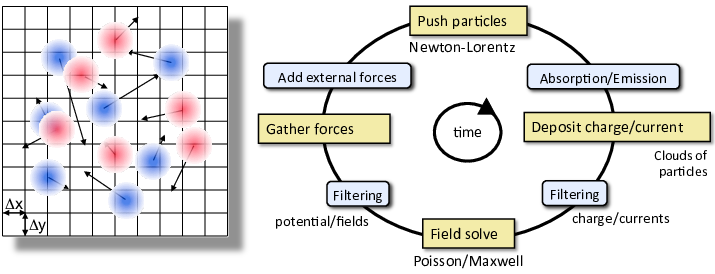
\includegraphics[scale=0.6]{figures/PIC.png}
%\par\end{centering}
\caption{\label{fig:PIC} The Particle-In-Cell (PIC) method follows the evolution of a collection of charged macro-particles (positively charged in blue on the left plot, negatively charged in red) that evolve self-consistently with their electromagnetic (or electrostatic) fields. The core PIC algorithm involves four operations at each time step: 1) evolve the velocity and position of the particles using the Newton-Lorentz equations, 2) deposit the charge and/or current densities through interpolation from the particles distributions onto the grid, 3) evolve Maxwell's wave equations (for electromagnetic) or solve Poisson's equation (for electrostatic) on the grid, 4) interpolate the fields from the grid onto the particles for the next particle push. Additional ``add-ons'' operations are inserted between these core operations to account for additional physics (e.g. absorption/emission of particles, addition of external forces to account for accelerator focusing or accelerating component) or numerical effects (e.g. smoothing/filtering of the charge/current densities and/or fields on the grid).}
\end{figure}

In the electromagnetic Particle-In-Cell method \cite{Birdsalllangdon},
the electromagnetic fields are solved on a grid, usually using Maxwell's
equations

\begin{subequations}
\begin{eqnarray}
\frac{\mathbf{\partial B}}{\partial t} & = & -\nabla\times\mathbf{E}\label{Eq:Faraday-1}\\
\frac{\mathbf{\partial E}}{\partial t} & = & \nabla\times\mathbf{B}-\mathbf{J}\label{Eq:Ampere-1}\\
\nabla\cdot\mathbf{E} & = & \rho\label{Eq:Gauss-1}\\
\nabla\cdot\mathbf{B} & = & 0\label{Eq:divb-1}
\end{eqnarray}
\end{subequations}
given here in natural units ($\epsilon_0=\mu_0=c=1$), where $t$ is time, $\mathbf{E}$ and
$\mathbf{B}$ are the electric and magnetic field components, and
$\rho$ and $\mathbf{J}$ are the charge and current densities. The
charged particles are advanced in time using the Newton-Lorentz equations
of motion 
\begin{subequations}
\begin{align}
\frac{d\mathbf{x}}{dt}= & \mathbf{v},\label{Eq:Lorentz_x-1}\\
\frac{d\left(\gamma\mathbf{v}\right)}{dt}= & \frac{q}{m}\left(\mathbf{E}+\mathbf{v}\times\mathbf{B}\right),\label{Eq:Lorentz_v-1}
\end{align}
\end{subequations}
where $m$, $q$, $\mathbf{x}$, $\mathbf{v}$ and $\gamma=1/\sqrt{1-v^{2}}$
 are respectively the mass, charge, position, velocity and relativistic
factor of the particle given in natural units ($c=1$). The charge and current densities are interpolated
on the grid from the particles' positions and velocities, while the
electric and magnetic field components are interpolated from the grid
to the particles' positions for the velocity update.

%%%%%%%%%%%%%%%%%%%%%%%%%%%%%%%%%%%
\subsection{Particle push}
%%%%%%%%%%%%%%%%%%%%%%%%%%%%%%%%%%%

A centered finite-difference discretization of the Newton-Lorentz
equations of motion is given by 
\begin{subequations}
\begin{align}
\frac{\mathbf{x}^{i+1}-\mathbf{x}^{i}}{\Delta t}= & \mathbf{v}^{i+1/2},\label{Eq:leapfrog_x}\\
\frac{\gamma^{i+1/2}\mathbf{v}^{i+1/2}-\gamma^{i-1/2}\mathbf{v}^{i-1/2}}{\Delta t}= & \frac{q}{m}\left(\mathbf{E}^{i}+\mathbf{\bar{v}}^{i}\times\mathbf{B}^{i}\right).\label{Eq:leapfrog_v}
\end{align}
\end{subequations}
In order to close the system, $\bar{\mathbf{v}}^{i}$ must be
expressed as a function of the other quantities. The two implementations that have become the most popular are presented below.

%%%%%%%%%%%%%%%%%%%%%%%%%%%%%%%%%%%
\subsubsection{Boris relativistic velocity rotation}
%%%%%%%%%%%%%%%%%%%%%%%%%%%%%%%%%%%
% Copyright 2017-2019 Jean-Luc Vay, Remi Lehe
%
% This file is part of WarpX.
%
% License: BSD-3-Clause-LBNL


\usepackage{bm}
\usepackage{amsmath}
\usepackage{amssymb}
\usepackage{graphicx}
\usepackage{url}
\usepackage{hyperref}

\usepackage[displaymath]{lineno}\usepackage{bm}% bold math

\newcommand{\fe}{\mathbf{\tilde{E}}}
\newcommand{\fb}{\mathbf{\tilde{B}}}
\newcommand{\fj}{\mathbf{\tilde{J}}}
\newcommand{\ff}{\tilde{F}}
\newcommand{\fg}{\tilde{G}}
\newcommand{\fk}{\mathbf{k}}
\newcommand{\fkhat}{\mathbf{\hat{k}}}

% Definitions from Remi's paper on Galilean math
\newcommand{\Km}{\vec{K}_{\vec{m}}}
\newcommand{\km}{\vec{k}_{\vec{m}}}
\renewcommand{\vec}[1]{\boldsymbol{#1}}
\newcommand{\vgal}{\vec{v}_{gal}}
\newcommand{\nab}{\vec{\nabla'}}
\newcommand{\Dt}[1]{ \frac{\partial #1}{\partial t}}
\newcommand{\mc}[1]{\hat{\mathcal{#1}}}
\newcommand{\xj}{\vec{x}'_{\vec{j}}}
\newcommand{\Xll}{\vec{X}_{\vec{\ell}}}
\newcommand{\Integ}[1]{\int_{-\infty}^{\infty} \!\!\!\!\!\!
  \mathrm{d}#1}
\newcommand{\RInteg}[1]{\int_{0}^{\infty} \!\! \frac{#1\mathrm{d}#1}{(2\pi)^2}}

% Definitions from Remi's Thesis
\newcommand{\h}{\mathcal{H}}
\newcommand{\hf}{\frac{1}{2}}
\newcommand{\um}{$\mu$m}
\newcommand{\Um}{\mu \mathrm{m}}
\newcommand{\aal}{\langle \vec{a}_l^2 \rangle}
\newcommand{\etad}{ \eta_d }
\newcommand{\etae}{ \eta_\epsilon }
\newcommand{\etag}{ \eta_\gamma }
\newcommand{\tlambda}{ \tilde{\lambda} }
%\newcommand\comment[1]{\textcolor{red}{\textbf{#1}}}
\newcommand{\gsim}{\mathrel{\hbox{\rlap{\lower.55ex
\hbox{$\sim$}} \kern-.3em \raise.4ex \hbox{$>$}}}}
\newcommand{\lsim}{\mathrel{\hbox{\rlap{\lower.55ex
\hbox{$\sim$}} \kern-.3em \raise.4ex \hbox{$<$}}}}
\newcommand{\kfoc}{k_\mathrm{foc}}
\newcommand{\bkfoc}{\bar{k}_\mathrm{foc}}
\newcommand{\xil}{\xi_{\mathrm{laser}}}

\newcommand{\Ex}[2]{{E_x}^{#1}_{#2}}
\newcommand{\Ey}[2]{{E_y}^{#1}_{#2}}
\newcommand{\Ez}[2]{{E_z}^{#1}_{#2}}
\newcommand{\Bx}[2]{{B_x}^{#1}_{#2}}
\newcommand{\By}[2]{{B_y}^{#1}_{#2}}
\newcommand{\Bz}[2]{{B_z}^{#1}_{#2}}
\newcommand{\Jx}[2]{{J_x}^{#1}_{#2}}
\newcommand{\Jy}[2]{{J_y}^{#1}_{#2}}
\newcommand{\Jz}[2]{{J_z}^{#1}_{#2}}

\newcommand{\tEr}[2]{\tilde{E_r}^{#1}_{#2}}
\newcommand{\tEt}[2]{\tilde{E_\theta}^{#1}_{#2}}
\newcommand{\tEz}[2]{\tilde{E_z}^{#1}_{#2}}
\newcommand{\tBr}[2]{\tilde{B_r}^{#1}_{#2}}
\newcommand{\tBt}[2]{\tilde{B_\theta}^{#1}_{#2}}
\newcommand{\tBz}[2]{\tilde{B_z}^{#1}_{#2}}
\newcommand{\tJr}[2]{\tilde{J_r}^{#1}_{#2}}
\newcommand{\tJt}[2]{\tilde{J_\theta}^{#1}_{#2}}
\newcommand{\tJz}[2]{\tilde{J_z}^{#1}_{#2}}

\newcommand{\CCirc}{\textsc{Calder Circ}}
\newcommand{\CCart}{\textsc{Calder 3D}}

The solution proposed by Boris \cite{BorisICNSP70} is given by 
\begin{align}
\mathbf{\bar{v}}^{i}= & \frac{\gamma^{i+1/2}\mathbf{v}^{i+1/2}+\gamma^{i-1/2}\mathbf{v}^{i-1/2}}{2\bar{\gamma}^{i}}.\label{Eq:boris_v}
\end{align}
where $\bar{\gamma}^{i}$ is defined by $\bar{\gamma}^{i} \equiv (\gamma^{i+1/2}+\gamma^{i-1/2} )/2$.

The system (\ref{Eq:leapfrog_v},\ref{Eq:boris_v}) is solved very
efficiently following Boris' method, where the electric field push
is decoupled from the magnetic push. Setting $\mathbf{u}=\gamma\mathbf{v}$, the
velocity is updated using the following sequence:

\begin{subequations}
\begin{align}
\mathbf{u^{-}}= & \mathbf{u}^{i-1/2}+\left(q\Delta t/2m\right)\mathbf{E}^{i}\\
\mathbf{u'}= & \mathbf{u}^{-}+\mathbf{u}^{-}\times\mathbf{t}\\
\mathbf{u}^{+}= & \mathbf{u}^{-}+\mathbf{u'}\times2\mathbf{t}/(1+t^{2})\\
\mathbf{u}^{i+1/2}= & \mathbf{u}^{+}+\left(q\Delta t/2m\right)\mathbf{E}^{i}
\end{align}
\end{subequations}
where $\mathbf{t}=\left(q\Delta
  t/2m\right)\mathbf{B}^{i}/\bar{\gamma}^{i}$ and where
$\bar{\gamma}^{i}$ can be calculated as $\bar{\gamma}^{i}=\sqrt{1+(\mathbf{u}^-/c)^2}$. 

The Boris implementation is second-order accurate, time-reversible and fast. Its implementation is very widespread and used in the vast majority of PIC codes.


%%%%%%%%%%%%%%%%%%%%%%%%%%%%%%%%%%%
\subsubsection{Vay Lorentz-invariant formulation}
%%%%%%%%%%%%%%%%%%%%%%%%%%%%%%%%%%%
% Copyright 2017-2019 Jean-Luc Vay, Remi Lehe
%
% This file is part of WarpX.
%
% License: BSD-3-Clause-LBNL


\usepackage{bm}
\usepackage{amsmath}
\usepackage{amssymb}
\usepackage{graphicx}
\usepackage{url}
\usepackage{hyperref}

\usepackage[displaymath]{lineno}\usepackage{bm}% bold math

\newcommand{\fe}{\mathbf{\tilde{E}}}
\newcommand{\fb}{\mathbf{\tilde{B}}}
\newcommand{\fj}{\mathbf{\tilde{J}}}
\newcommand{\ff}{\tilde{F}}
\newcommand{\fg}{\tilde{G}}
\newcommand{\fk}{\mathbf{k}}
\newcommand{\fkhat}{\mathbf{\hat{k}}}

% Definitions from Remi's paper on Galilean math
\newcommand{\Km}{\vec{K}_{\vec{m}}}
\newcommand{\km}{\vec{k}_{\vec{m}}}
\renewcommand{\vec}[1]{\boldsymbol{#1}}
\newcommand{\vgal}{\vec{v}_{gal}}
\newcommand{\nab}{\vec{\nabla'}}
\newcommand{\Dt}[1]{ \frac{\partial #1}{\partial t}}
\newcommand{\mc}[1]{\hat{\mathcal{#1}}}
\newcommand{\xj}{\vec{x}'_{\vec{j}}}
\newcommand{\Xll}{\vec{X}_{\vec{\ell}}}
\newcommand{\Integ}[1]{\int_{-\infty}^{\infty} \!\!\!\!\!\!
  \mathrm{d}#1}
\newcommand{\RInteg}[1]{\int_{0}^{\infty} \!\! \frac{#1\mathrm{d}#1}{(2\pi)^2}}

% Definitions from Remi's Thesis
\newcommand{\h}{\mathcal{H}}
\newcommand{\hf}{\frac{1}{2}}
\newcommand{\um}{$\mu$m}
\newcommand{\Um}{\mu \mathrm{m}}
\newcommand{\aal}{\langle \vec{a}_l^2 \rangle}
\newcommand{\etad}{ \eta_d }
\newcommand{\etae}{ \eta_\epsilon }
\newcommand{\etag}{ \eta_\gamma }
\newcommand{\tlambda}{ \tilde{\lambda} }
%\newcommand\comment[1]{\textcolor{red}{\textbf{#1}}}
\newcommand{\gsim}{\mathrel{\hbox{\rlap{\lower.55ex
\hbox{$\sim$}} \kern-.3em \raise.4ex \hbox{$>$}}}}
\newcommand{\lsim}{\mathrel{\hbox{\rlap{\lower.55ex
\hbox{$\sim$}} \kern-.3em \raise.4ex \hbox{$<$}}}}
\newcommand{\kfoc}{k_\mathrm{foc}}
\newcommand{\bkfoc}{\bar{k}_\mathrm{foc}}
\newcommand{\xil}{\xi_{\mathrm{laser}}}

\newcommand{\Ex}[2]{{E_x}^{#1}_{#2}}
\newcommand{\Ey}[2]{{E_y}^{#1}_{#2}}
\newcommand{\Ez}[2]{{E_z}^{#1}_{#2}}
\newcommand{\Bx}[2]{{B_x}^{#1}_{#2}}
\newcommand{\By}[2]{{B_y}^{#1}_{#2}}
\newcommand{\Bz}[2]{{B_z}^{#1}_{#2}}
\newcommand{\Jx}[2]{{J_x}^{#1}_{#2}}
\newcommand{\Jy}[2]{{J_y}^{#1}_{#2}}
\newcommand{\Jz}[2]{{J_z}^{#1}_{#2}}

\newcommand{\tEr}[2]{\tilde{E_r}^{#1}_{#2}}
\newcommand{\tEt}[2]{\tilde{E_\theta}^{#1}_{#2}}
\newcommand{\tEz}[2]{\tilde{E_z}^{#1}_{#2}}
\newcommand{\tBr}[2]{\tilde{B_r}^{#1}_{#2}}
\newcommand{\tBt}[2]{\tilde{B_\theta}^{#1}_{#2}}
\newcommand{\tBz}[2]{\tilde{B_z}^{#1}_{#2}}
\newcommand{\tJr}[2]{\tilde{J_r}^{#1}_{#2}}
\newcommand{\tJt}[2]{\tilde{J_\theta}^{#1}_{#2}}
\newcommand{\tJz}[2]{\tilde{J_z}^{#1}_{#2}}

\newcommand{\CCirc}{\textsc{Calder Circ}}
\newcommand{\CCart}{\textsc{Calder 3D}}

It was shown in \cite{VayPOP2008} that the Boris formulation is
not Lorentz invariant and can lead to significant errors in the treatment
of relativistic dynamics. A Lorentz invariant formulation is obtained
by considering the following velocity average 
\begin{align}
\mathbf{\bar{v}}^{i}= & \frac{\mathbf{v}^{i+1/2}+\mathbf{v}^{i-1/2}}{2},\label{Eq:new_v}
\end{align}
This gives a system that is solvable analytically (see \cite{VayPOP2008}
for a detailed derivation), giving the following velocity update:

\begin{subequations}
\begin{align}
\mathbf{u^{*}}= & \mathbf{u}^{i-1/2}+\frac{q\Delta t}{m}\left(\mathbf{E}^{i}+\frac{\mathbf{v}^{i-1/2}}{2}\times\mathbf{B}^{i}\right),\label{pusher_gamma}\\
\mathbf{u}^{i+1/2}= & \left[\mathbf{u^{*}}+\left(\mathbf{u^{*}}\cdot\mathbf{t}\right)\mathbf{t}+\mathbf{u^{*}}\times\mathbf{t}\right]/\left(1+t^{2}\right),\label{pusher_upr}
\end{align}
\end{subequations}
where $\mathbf{t}=\bm{\tau}/\gamma^{i+1/2}$, $\bm{\tau}=\left(q\Delta t/2m\right)\mathbf{B}^{i}$,
$\gamma^{i+1/2}=\sqrt{\sigma+\sqrt{\sigma^{2}+\left(\tau^{2}+w^{2}\right)}}$,
$w=\mathbf{u^{*}}\cdot\bm{\tau}$, $\sigma=\left(\gamma'^{2}-\tau^{2}\right)/2$
and $\gamma'=\sqrt{1+(\mathbf{u}^{*}/c)^{2}}$. This Lorentz invariant formulation
is particularly well suited for the modeling of ultra-relativistic
charged particle beams, where the accurate account of the cancellation
of the self-generated electric and magnetic fields is essential, as
shown in \cite{VayPOP2008}.


%%%%%%%%%%%%%%%%%%%%%%%%%%%%%%%%%%%
\subsection{Field solve}
%%%%%%%%%%%%%%%%%%%%%%%%%%%%%%%%%%%

Various methods are available for solving Maxwell's equations on a
grid, based on finite-differences, finite-volume, finite-element,
spectral, or other discretization techniques that apply most commonly
on single structured or unstructured meshes and less commonly on multiblock
multiresolution grid structures. In this chapter, we summarize the widespread
second order finite-difference time-domain (FDTD) algorithm, its extension
to non-standard finite-differences as well as the pseudo-spectral
analytical time-domain (PSATD) and pseudo-spectral time-domain (PSTD)
algorithms. Extension to multiresolution (or mesh refinement) PIC
is described in, e.g. \cite{VayCSD12,Vaycpc04}.

%%%%%%%%%%%%%%%%%%%%%%%%%%%%%%%%%%%
\subsubsection{Finite-Difference Time-Domain (FDTD)}
%%%%%%%%%%%%%%%%%%%%%%%%%%%%%%%%%%%
% Copyright 2017-2019 Jean-Luc Vay, Remi Lehe
%
% This file is part of WarpX.
%
% License: BSD-3-Clause-LBNL


\usepackage{bm}
\usepackage{amsmath}
\usepackage{amssymb}
\usepackage{graphicx}
\usepackage{url}
\usepackage{hyperref}

\usepackage[displaymath]{lineno}\usepackage{bm}% bold math

\newcommand{\fe}{\mathbf{\tilde{E}}}
\newcommand{\fb}{\mathbf{\tilde{B}}}
\newcommand{\fj}{\mathbf{\tilde{J}}}
\newcommand{\ff}{\tilde{F}}
\newcommand{\fg}{\tilde{G}}
\newcommand{\fk}{\mathbf{k}}
\newcommand{\fkhat}{\mathbf{\hat{k}}}

% Definitions from Remi's paper on Galilean math
\newcommand{\Km}{\vec{K}_{\vec{m}}}
\newcommand{\km}{\vec{k}_{\vec{m}}}
\renewcommand{\vec}[1]{\boldsymbol{#1}}
\newcommand{\vgal}{\vec{v}_{gal}}
\newcommand{\nab}{\vec{\nabla'}}
\newcommand{\Dt}[1]{ \frac{\partial #1}{\partial t}}
\newcommand{\mc}[1]{\hat{\mathcal{#1}}}
\newcommand{\xj}{\vec{x}'_{\vec{j}}}
\newcommand{\Xll}{\vec{X}_{\vec{\ell}}}
\newcommand{\Integ}[1]{\int_{-\infty}^{\infty} \!\!\!\!\!\!
  \mathrm{d}#1}
\newcommand{\RInteg}[1]{\int_{0}^{\infty} \!\! \frac{#1\mathrm{d}#1}{(2\pi)^2}}

% Definitions from Remi's Thesis
\newcommand{\h}{\mathcal{H}}
\newcommand{\hf}{\frac{1}{2}}
\newcommand{\um}{$\mu$m}
\newcommand{\Um}{\mu \mathrm{m}}
\newcommand{\aal}{\langle \vec{a}_l^2 \rangle}
\newcommand{\etad}{ \eta_d }
\newcommand{\etae}{ \eta_\epsilon }
\newcommand{\etag}{ \eta_\gamma }
\newcommand{\tlambda}{ \tilde{\lambda} }
%\newcommand\comment[1]{\textcolor{red}{\textbf{#1}}}
\newcommand{\gsim}{\mathrel{\hbox{\rlap{\lower.55ex
\hbox{$\sim$}} \kern-.3em \raise.4ex \hbox{$>$}}}}
\newcommand{\lsim}{\mathrel{\hbox{\rlap{\lower.55ex
\hbox{$\sim$}} \kern-.3em \raise.4ex \hbox{$<$}}}}
\newcommand{\kfoc}{k_\mathrm{foc}}
\newcommand{\bkfoc}{\bar{k}_\mathrm{foc}}
\newcommand{\xil}{\xi_{\mathrm{laser}}}

\newcommand{\Ex}[2]{{E_x}^{#1}_{#2}}
\newcommand{\Ey}[2]{{E_y}^{#1}_{#2}}
\newcommand{\Ez}[2]{{E_z}^{#1}_{#2}}
\newcommand{\Bx}[2]{{B_x}^{#1}_{#2}}
\newcommand{\By}[2]{{B_y}^{#1}_{#2}}
\newcommand{\Bz}[2]{{B_z}^{#1}_{#2}}
\newcommand{\Jx}[2]{{J_x}^{#1}_{#2}}
\newcommand{\Jy}[2]{{J_y}^{#1}_{#2}}
\newcommand{\Jz}[2]{{J_z}^{#1}_{#2}}

\newcommand{\tEr}[2]{\tilde{E_r}^{#1}_{#2}}
\newcommand{\tEt}[2]{\tilde{E_\theta}^{#1}_{#2}}
\newcommand{\tEz}[2]{\tilde{E_z}^{#1}_{#2}}
\newcommand{\tBr}[2]{\tilde{B_r}^{#1}_{#2}}
\newcommand{\tBt}[2]{\tilde{B_\theta}^{#1}_{#2}}
\newcommand{\tBz}[2]{\tilde{B_z}^{#1}_{#2}}
\newcommand{\tJr}[2]{\tilde{J_r}^{#1}_{#2}}
\newcommand{\tJt}[2]{\tilde{J_\theta}^{#1}_{#2}}
\newcommand{\tJz}[2]{\tilde{J_z}^{#1}_{#2}}

\newcommand{\CCirc}{\textsc{Calder Circ}}
\newcommand{\CCart}{\textsc{Calder 3D}}

The most popular algorithm for electromagnetic PIC codes is the Finite-Difference
Time-Domain (or FDTD) solver

\begin{subequations}
\begin{eqnarray}
D_{t}\mathbf{B} & = & -\nabla\times\mathbf{E}\label{Eq:Faraday-2}\\
D_{t}\mathbf{E} & = & \nabla\times\mathbf{B}-\mathbf{J}\label{Eq:Ampere-2}\\
\left[\nabla\cdot\mathbf{E}\right. & = & \left.\rho\right]\label{Eq:Gauss-2}\\
\left[\nabla\cdot\mathbf{B}\right. & = & \left.0\right].\label{Eq:divb-2}
\end{eqnarray}
\end{subequations}

\begin{figure}
%\begin{centering}
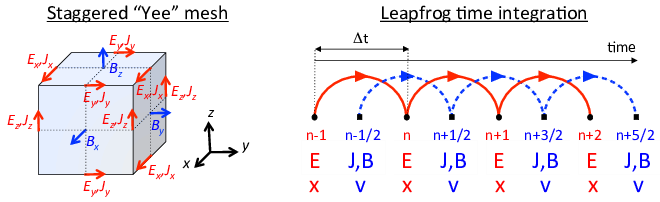
\includegraphics[scale=0.7]{Yee_grid.png}
%\par\end{centering}
\caption{\label{fig:yee_grid}(left) Layout of field components on the staggered ``Yee'' grid. Current densities and electric fields are defined on the edges of the cells and magnetic fields on the faces. (right) Time integration using a second-order finite-difference "leapfrog" integrator.}
\end{figure}

The differential operator is defined as $\nabla=D_{x}\mathbf{\hat{x}}+D_{y}\mathbf{\hat{y}}+D_{z}\mathbf{\hat{z}}$
and the finite-difference operators in time and space are defined
respectively as $ $$D_{t}G|_{i,j,k}^{n}=\left(G|_{i,j,k}^{n+1/2}-G|_{i,j,k}^{n-1/2}\right)/\Delta t$$ $
and $D_{x}G|_{i,j,k}^{n}=\left(G|_{i+1/2,j,k}^{n}-G|_{i-1/2,j,k}^{n}\right)/\Delta x$,
where $\Delta t$ and $\Delta x$ are respectively the time step and
the grid cell size along $x$, $n$ is the time index and $i$, $j$
and $k$ are the spatial indices along $x$, $y$ and $z$ respectively.
The difference operators along $y$ and $z$ are obtained by circular
permutation. The equations in brackets are given for completeness,
as they are often not actually solved, thanks to the usage of a so-called
charge conserving algorithm, as explained below. As shown in Figure
\ref{fig:yee_grid}, the quantities are given on a staggered (or ``Yee'')
grid \cite{Yee}, where the electric field components are located
between nodes and the magnetic field components are located in the
center of the cell faces. Knowing the current densities at half-integer steps, 
the electric field components are updated alternately with the magnetic 
field components at integer and half-integer steps respectively.


%%%%%%%%%%%%%%%%%%%%%%%%%%%%%%%%%%%
\subsubsection{Non-Standard Finite-Difference Time-Domain (NSFDTD)}
%%%%%%%%%%%%%%%%%%%%%%%%%%%%%%%%%%%
% Copyright 2017-2019 Jean-Luc Vay, Remi Lehe
%
% This file is part of WarpX.
%
% License: BSD-3-Clause-LBNL


\usepackage{bm}
\usepackage{amsmath}
\usepackage{amssymb}
\usepackage{graphicx}
\usepackage{url}
\usepackage{hyperref}

\usepackage[displaymath]{lineno}\usepackage{bm}% bold math

\newcommand{\fe}{\mathbf{\tilde{E}}}
\newcommand{\fb}{\mathbf{\tilde{B}}}
\newcommand{\fj}{\mathbf{\tilde{J}}}
\newcommand{\ff}{\tilde{F}}
\newcommand{\fg}{\tilde{G}}
\newcommand{\fk}{\mathbf{k}}
\newcommand{\fkhat}{\mathbf{\hat{k}}}

% Definitions from Remi's paper on Galilean math
\newcommand{\Km}{\vec{K}_{\vec{m}}}
\newcommand{\km}{\vec{k}_{\vec{m}}}
\renewcommand{\vec}[1]{\boldsymbol{#1}}
\newcommand{\vgal}{\vec{v}_{gal}}
\newcommand{\nab}{\vec{\nabla'}}
\newcommand{\Dt}[1]{ \frac{\partial #1}{\partial t}}
\newcommand{\mc}[1]{\hat{\mathcal{#1}}}
\newcommand{\xj}{\vec{x}'_{\vec{j}}}
\newcommand{\Xll}{\vec{X}_{\vec{\ell}}}
\newcommand{\Integ}[1]{\int_{-\infty}^{\infty} \!\!\!\!\!\!
  \mathrm{d}#1}
\newcommand{\RInteg}[1]{\int_{0}^{\infty} \!\! \frac{#1\mathrm{d}#1}{(2\pi)^2}}

% Definitions from Remi's Thesis
\newcommand{\h}{\mathcal{H}}
\newcommand{\hf}{\frac{1}{2}}
\newcommand{\um}{$\mu$m}
\newcommand{\Um}{\mu \mathrm{m}}
\newcommand{\aal}{\langle \vec{a}_l^2 \rangle}
\newcommand{\etad}{ \eta_d }
\newcommand{\etae}{ \eta_\epsilon }
\newcommand{\etag}{ \eta_\gamma }
\newcommand{\tlambda}{ \tilde{\lambda} }
%\newcommand\comment[1]{\textcolor{red}{\textbf{#1}}}
\newcommand{\gsim}{\mathrel{\hbox{\rlap{\lower.55ex
\hbox{$\sim$}} \kern-.3em \raise.4ex \hbox{$>$}}}}
\newcommand{\lsim}{\mathrel{\hbox{\rlap{\lower.55ex
\hbox{$\sim$}} \kern-.3em \raise.4ex \hbox{$<$}}}}
\newcommand{\kfoc}{k_\mathrm{foc}}
\newcommand{\bkfoc}{\bar{k}_\mathrm{foc}}
\newcommand{\xil}{\xi_{\mathrm{laser}}}

\newcommand{\Ex}[2]{{E_x}^{#1}_{#2}}
\newcommand{\Ey}[2]{{E_y}^{#1}_{#2}}
\newcommand{\Ez}[2]{{E_z}^{#1}_{#2}}
\newcommand{\Bx}[2]{{B_x}^{#1}_{#2}}
\newcommand{\By}[2]{{B_y}^{#1}_{#2}}
\newcommand{\Bz}[2]{{B_z}^{#1}_{#2}}
\newcommand{\Jx}[2]{{J_x}^{#1}_{#2}}
\newcommand{\Jy}[2]{{J_y}^{#1}_{#2}}
\newcommand{\Jz}[2]{{J_z}^{#1}_{#2}}

\newcommand{\tEr}[2]{\tilde{E_r}^{#1}_{#2}}
\newcommand{\tEt}[2]{\tilde{E_\theta}^{#1}_{#2}}
\newcommand{\tEz}[2]{\tilde{E_z}^{#1}_{#2}}
\newcommand{\tBr}[2]{\tilde{B_r}^{#1}_{#2}}
\newcommand{\tBt}[2]{\tilde{B_\theta}^{#1}_{#2}}
\newcommand{\tBz}[2]{\tilde{B_z}^{#1}_{#2}}
\newcommand{\tJr}[2]{\tilde{J_r}^{#1}_{#2}}
\newcommand{\tJt}[2]{\tilde{J_\theta}^{#1}_{#2}}
\newcommand{\tJz}[2]{\tilde{J_z}^{#1}_{#2}}

\newcommand{\CCirc}{\textsc{Calder Circ}}
\newcommand{\CCart}{\textsc{Calder 3D}}

In \cite{Coleieee1997,Coleieee2002}, Cole introduced an implementation
of the source-free Maxwell's wave equations for narrow-band applications
based on non-standard finite-differences (NSFD). In \cite{Karkicap06},
Karkkainen \emph{et al.} adapted it for wideband applications. At
the Courant limit for the time step and for a given set of parameters,
the stencil proposed in \cite{Karkicap06} has no numerical dispersion
along the principal axes, provided that the cell size is the same
along each dimension (i.e. cubic cells in 3D). The ``Cole-Karkkainnen''
(or CK) solver uses the non-standard finite difference formulation
(based on extended stencils) of the Maxwell-Ampere equation and can be 
implemented as follows \cite{Vayjcp2011}:

\begin{subequations}
\begin{eqnarray}
D_{t}\mathbf{B} & = & -\nabla^{*}\times\mathbf{E}\label{Eq:Faraday}\\
D_{t}\mathbf{E} & = & \nabla\times\mathbf{B}-\mathbf{J}\label{Eq:Ampere}\\
\left[\nabla\cdot\mathbf{E}\right. & = & \left.\rho\right]\label{Eq:Gauss}\\
\left[\nabla^{*}\cdot\mathbf{B}\right. & = & \left.0\right]\label{Eq:divb}
\end{eqnarray}
\end{subequations}

Eq. \ref{Eq:Gauss} and \ref{Eq:divb} are not being solved explicitly
but verified via appropriate initial conditions and current deposition
procedure. The NSFD differential operators is given by $\nabla^{*}=D_{x}^{*}\mathbf{\hat{x}}+D_{y}^{*}\mathbf{\hat{y}}+D_{z}^{*}\mathbf{\hat{z}}$
where $D_{x}^{*}=\left(\alpha+\beta S_{x}^{1}+\xi S_{x}^{2}\right)D_{x}$
with $S_{x}^{1}G|_{i,j,k}^{n}=G|_{i,j+1,k}^{n}+G|_{i,j-1,k}^{n}+G|_{i,j,k+1}^{n}+G|_{i,j,k-1}^{n}$,
$S_{x}^{2}G|_{i,j,k}^{n}=G|_{i,j+1,k+1}^{n}+G|_{i,j-1,k+1}^{n}+G|_{i,j+1,k-1}^{n}+G|_{i,j-1,k-1}^{n}$.
$G$ is a sample vector component, while $\alpha$, $\beta$ and $\xi$
are constant scalars satisfying $\alpha+4\beta+4\xi=1$. As with
the FDTD algorithm, the quantities with half-integer are located between
the nodes (electric field components) or in the center of the cell
faces (magnetic field components). The operators along $y$ and $z$,
i.e. $D_{y}$, $D_{z}$, $D_{y}^{*}$, $D_{z}^{*}$, $S_{y}^{1}$,
$S_{z}^{1}$, $S_{y}^{2}$, and $S_{z}^{2}$, are obtained by circular
permutation of the indices.

Assuming cubic cells ($\Delta x=\Delta y=\Delta z$), the coefficients
given in \cite{Karkicap06} ($\alpha=7/12$, $\beta=1/12$ and $\xi=1/48$)
allow for the Courant condition to be at $\Delta t=\Delta x$, which
equates to having no numerical dispersion along the principal axes.
The algorithm reduces to the FDTD algorithm with $\alpha=1$ and $\beta=\xi=0$.
An extension to non-cubic cells is provided by Cowan, \emph{et al.}
in 3-D in \cite{CowanPRSTAB13} and was given by Pukhov in 2-D in
\cite{PukhovJPP99}. An alternative NSFDTD implementation that enables superluminous waves is also
given by Lehe {\it et al.} in \cite{LehePRSTAB13}. 

As mentioned above, a key feature of the algorithms based on NSFDTD
is that some implementations \cite{Karkicap06,CowanPRSTAB13} enable the time step $\Delta t=\Delta x$ along one or
more axes and no numerical dispersion along those axes. However, as
shown in \cite{Vayjcp2011}, an instability develops at the Nyquist
wavelength at (or very near) such a timestep. It is also shown in
the same paper that removing the Nyquist component in all the source
terms using a bilinear filter (see description of the filter below)
suppresses this instability.



%%%%%%%%%%%%%%%%%%%%%%%%%%%%%%%%%%%
\subsubsection{Pseudo Spectral Analytical Time Domain (PSATD)}
%%%%%%%%%%%%%%%%%%%%%%%%%%%%%%%%%%%
% Copyright 2017-2019 Jean-Luc Vay, Remi Lehe
%
% This file is part of WarpX.
%
% License: BSD-3-Clause-LBNL


\usepackage{bm}
\usepackage{amsmath}
\usepackage{amssymb}
\usepackage{graphicx}
\usepackage{url}
\usepackage{hyperref}

\usepackage[displaymath]{lineno}\usepackage{bm}% bold math

\newcommand{\fe}{\mathbf{\tilde{E}}}
\newcommand{\fb}{\mathbf{\tilde{B}}}
\newcommand{\fj}{\mathbf{\tilde{J}}}
\newcommand{\ff}{\tilde{F}}
\newcommand{\fg}{\tilde{G}}
\newcommand{\fk}{\mathbf{k}}
\newcommand{\fkhat}{\mathbf{\hat{k}}}

% Definitions from Remi's paper on Galilean math
\newcommand{\Km}{\vec{K}_{\vec{m}}}
\newcommand{\km}{\vec{k}_{\vec{m}}}
\renewcommand{\vec}[1]{\boldsymbol{#1}}
\newcommand{\vgal}{\vec{v}_{gal}}
\newcommand{\nab}{\vec{\nabla'}}
\newcommand{\Dt}[1]{ \frac{\partial #1}{\partial t}}
\newcommand{\mc}[1]{\hat{\mathcal{#1}}}
\newcommand{\xj}{\vec{x}'_{\vec{j}}}
\newcommand{\Xll}{\vec{X}_{\vec{\ell}}}
\newcommand{\Integ}[1]{\int_{-\infty}^{\infty} \!\!\!\!\!\!
  \mathrm{d}#1}
\newcommand{\RInteg}[1]{\int_{0}^{\infty} \!\! \frac{#1\mathrm{d}#1}{(2\pi)^2}}

% Definitions from Remi's Thesis
\newcommand{\h}{\mathcal{H}}
\newcommand{\hf}{\frac{1}{2}}
\newcommand{\um}{$\mu$m}
\newcommand{\Um}{\mu \mathrm{m}}
\newcommand{\aal}{\langle \vec{a}_l^2 \rangle}
\newcommand{\etad}{ \eta_d }
\newcommand{\etae}{ \eta_\epsilon }
\newcommand{\etag}{ \eta_\gamma }
\newcommand{\tlambda}{ \tilde{\lambda} }
%\newcommand\comment[1]{\textcolor{red}{\textbf{#1}}}
\newcommand{\gsim}{\mathrel{\hbox{\rlap{\lower.55ex
\hbox{$\sim$}} \kern-.3em \raise.4ex \hbox{$>$}}}}
\newcommand{\lsim}{\mathrel{\hbox{\rlap{\lower.55ex
\hbox{$\sim$}} \kern-.3em \raise.4ex \hbox{$<$}}}}
\newcommand{\kfoc}{k_\mathrm{foc}}
\newcommand{\bkfoc}{\bar{k}_\mathrm{foc}}
\newcommand{\xil}{\xi_{\mathrm{laser}}}

\newcommand{\Ex}[2]{{E_x}^{#1}_{#2}}
\newcommand{\Ey}[2]{{E_y}^{#1}_{#2}}
\newcommand{\Ez}[2]{{E_z}^{#1}_{#2}}
\newcommand{\Bx}[2]{{B_x}^{#1}_{#2}}
\newcommand{\By}[2]{{B_y}^{#1}_{#2}}
\newcommand{\Bz}[2]{{B_z}^{#1}_{#2}}
\newcommand{\Jx}[2]{{J_x}^{#1}_{#2}}
\newcommand{\Jy}[2]{{J_y}^{#1}_{#2}}
\newcommand{\Jz}[2]{{J_z}^{#1}_{#2}}

\newcommand{\tEr}[2]{\tilde{E_r}^{#1}_{#2}}
\newcommand{\tEt}[2]{\tilde{E_\theta}^{#1}_{#2}}
\newcommand{\tEz}[2]{\tilde{E_z}^{#1}_{#2}}
\newcommand{\tBr}[2]{\tilde{B_r}^{#1}_{#2}}
\newcommand{\tBt}[2]{\tilde{B_\theta}^{#1}_{#2}}
\newcommand{\tBz}[2]{\tilde{B_z}^{#1}_{#2}}
\newcommand{\tJr}[2]{\tilde{J_r}^{#1}_{#2}}
\newcommand{\tJt}[2]{\tilde{J_\theta}^{#1}_{#2}}
\newcommand{\tJz}[2]{\tilde{J_z}^{#1}_{#2}}

\newcommand{\CCirc}{\textsc{Calder Circ}}
\newcommand{\CCart}{\textsc{Calder 3D}}

Maxwell's equations in Fourier space are given by % --- Maxwell
\begin{subequations}
\begin{eqnarray}
\frac{\partial\fe}{\partial t} & = & i\fk\times\fb-\fj\\
\frac{\partial\fb}{\partial t} & = & -i\fk\times\fe\\
{}[i\fk\cdot\fe & = & \tilde{\rho}]\\
{}[i\fk\cdot\fb & = & 0]
\end{eqnarray}
\end{subequations}
where $\tilde{a}$ is the Fourier Transform of the quantity $a$.
As with the real space formulation, provided that the continuity equation
$\partial\tilde{\rho}/\partial t+i\fk\cdot\fj=0$ is satisfied, then
the last two equations will automatically be satisfied at any time
if satisfied initially and do not need to be explicitly integrated.

Decomposing the electric field and current between longitudinal and
transverse components $\fe=\fe_{L}+\fe_{T}=\fkhat(\fkhat\cdot\fe)-\fkhat\times(\fkhat\times\fe)$
and $\fj=\fj_{L}+\fj_{T}=\fkhat(\fkhat\cdot\fj)-\fkhat\times(\fkhat\times\fj)$
gives
\begin{subequations}
\begin{eqnarray}
\frac{\partial\fe_{T}}{\partial t} & = & i\fk\times\fb-\mathbf{\tilde{J}_{T}}\\
\frac{\partial\fe_{L}}{\partial t} & = & -\mathbf{\tilde{J}_{L}}\\
\frac{\partial\fb}{\partial t} & = & -i\fk\times\fe
\end{eqnarray}
\end{subequations}
with $\fkhat=\fk/k$.

If the sources are assumed to be constant over a time interval $\Delta t$,
the system of equations is solvable analytically and is given by (see
\cite{Habericnsp73} for the original formulation and \cite{VayJCP13}
for a more detailed derivation):

% --- PSATD
\begin{subequations}
\label{Eq:PSATD}
\begin{eqnarray}
\fe_{T}^{n+1} & = & C\fe_{T}^{n}+iS\fkhat\times\fb^{n}-\frac{S}{k}\fj_{T}^{n+1/2}\label{Eq:PSATD_transverse_1}\\
\fe_{L}^{n+1} & = & \fe_{L}^{n}-\Delta t\fj_{L}^{n+1/2}\\
\fb^{n+1} & = & C\fb^{n}-iS\fkhat\times\fe^{n}\\
&+&i\frac{1-C}{k}\fkhat\times\fj^{n+1/2}\label{Eq:PSATD_transverse_2}
\end{eqnarray}
\end{subequations}
with $C=\cos\left(k\Delta t\right)$ and $S=\sin\left(k\Delta t\right)$.

Combining the transverse and longitudinal components, gives 
\begin{subequations}
\begin{eqnarray}
\fe^{n+1} & = & C\fe^{n}+iS\fkhat\times\fb^{n}-\frac{S}{k}\fj^{n+1/2}\\
 & + &(1-C)\fkhat(\fkhat\cdot\fe^{n})\nonumber \\
 & + & \fkhat(\fkhat\cdot\fj^{n+1/2})\left(\frac{S}{k}-\Delta t\right),\label{Eq_PSATD_1}\\
\fb^{n+1} & = & C\fb^{n}-iS\fkhat\times\fe^{n}\\
&+&i\frac{1-C}{k}\fkhat\times\fj^{n+1/2}.\label{Eq_PSATD_2}
\end{eqnarray}
\end{subequations}

For fields generated by the source terms without the self-consistent
dynamics of the charged particles, this algorithm is free of numerical
dispersion and is not subject to a Courant condition. Furthermore,
this solution is exact for any time step size subject to the assumption
that the current source is constant over that time step. 

As shown in \cite{VayJCP13}, by expanding the coefficients $S_{h}$
and $C_{h}$ in Taylor series and keeping the leading terms, the PSATD
formulation reduces to the perhaps better known pseudo-spectral time-domain
(PSTD) formulation \cite{DawsonRMP83,Liumotl1997}: % --- PSTD
\begin{subequations}
\begin{eqnarray}
\fe^{n+1} & = & \fe^{n}+i\Delta t\fk\times\fb^{n+1/2}-\Delta t\fj^{n+1/2},\\
\fb^{n+3/2} & = & \fb^{n+1/2}-i\Delta t\fk\times\fe^{n+1}.
\end{eqnarray}
\end{subequations}
The dispersion relation of the PSTD solver is given by $\sin(\frac{\omega\Delta t}{2})=\frac{k\Delta t}{2}.$
In contrast to the PSATD solver, the PSTD solver is subject to numerical
dispersion for a finite time step and to a Courant condition that
is given by $\Delta t\leq \frac{2}{\pi}\left(\frac{1}{\Delta x^{2}}+\frac{1}{\Delta y^{2}}+\frac{1}{\Delta x^{2}}\right)^{-1/2}.$

The PSATD and PSTD formulations that were just given apply to the
field components located at the nodes of the grid. As noted in \cite{Ohmurapiers2010},
they can also be easily recast on a staggered Yee grid by multiplication
of the field components by the appropriate phase factors to shift
them from the collocated to the staggered locations. The choice between
a collocated and a staggered formulation is application-dependent.

Spectral solvers used to be very popular in the years 1970s to early 1990s, before being replaced by finite-difference methods with the advent of parallel supercomputers that favored local methods. However, it was shown recently that standard domain decomposition with Fast Fourier Transforms that are local to each subdomain could be used effectively with PIC spectral methods \cite{VayJCP13}, at the cost of truncation errors in the guard cells that could be neglected. A detailed analysis of the effectiveness of the method with exact evaluation of the magnitude of the effect of the truncation error is given in \cite{Vincenti2016a} for stencils of arbitrary order (up-to the infinite ``spectral'' order).


%%%%%%%%%%%%%%%%%%%%%%%%%%%%%%%%%%%
\subsection{Current deposition}
%%%%%%%%%%%%%%%%%%%%%%%%%%%%%%%%%%%
% Copyright 2017-2019 Jean-Luc Vay, Remi Lehe
%
% This file is part of WarpX.
%
% License: BSD-3-Clause-LBNL


\usepackage{bm}
\usepackage{amsmath}
\usepackage{amssymb}
\usepackage{graphicx}
\usepackage{url}
\usepackage{hyperref}

\usepackage[displaymath]{lineno}\usepackage{bm}% bold math

\newcommand{\fe}{\mathbf{\tilde{E}}}
\newcommand{\fb}{\mathbf{\tilde{B}}}
\newcommand{\fj}{\mathbf{\tilde{J}}}
\newcommand{\ff}{\tilde{F}}
\newcommand{\fg}{\tilde{G}}
\newcommand{\fk}{\mathbf{k}}
\newcommand{\fkhat}{\mathbf{\hat{k}}}

% Definitions from Remi's paper on Galilean math
\newcommand{\Km}{\vec{K}_{\vec{m}}}
\newcommand{\km}{\vec{k}_{\vec{m}}}
\renewcommand{\vec}[1]{\boldsymbol{#1}}
\newcommand{\vgal}{\vec{v}_{gal}}
\newcommand{\nab}{\vec{\nabla'}}
\newcommand{\Dt}[1]{ \frac{\partial #1}{\partial t}}
\newcommand{\mc}[1]{\hat{\mathcal{#1}}}
\newcommand{\xj}{\vec{x}'_{\vec{j}}}
\newcommand{\Xll}{\vec{X}_{\vec{\ell}}}
\newcommand{\Integ}[1]{\int_{-\infty}^{\infty} \!\!\!\!\!\!
  \mathrm{d}#1}
\newcommand{\RInteg}[1]{\int_{0}^{\infty} \!\! \frac{#1\mathrm{d}#1}{(2\pi)^2}}

% Definitions from Remi's Thesis
\newcommand{\h}{\mathcal{H}}
\newcommand{\hf}{\frac{1}{2}}
\newcommand{\um}{$\mu$m}
\newcommand{\Um}{\mu \mathrm{m}}
\newcommand{\aal}{\langle \vec{a}_l^2 \rangle}
\newcommand{\etad}{ \eta_d }
\newcommand{\etae}{ \eta_\epsilon }
\newcommand{\etag}{ \eta_\gamma }
\newcommand{\tlambda}{ \tilde{\lambda} }
%\newcommand\comment[1]{\textcolor{red}{\textbf{#1}}}
\newcommand{\gsim}{\mathrel{\hbox{\rlap{\lower.55ex
\hbox{$\sim$}} \kern-.3em \raise.4ex \hbox{$>$}}}}
\newcommand{\lsim}{\mathrel{\hbox{\rlap{\lower.55ex
\hbox{$\sim$}} \kern-.3em \raise.4ex \hbox{$<$}}}}
\newcommand{\kfoc}{k_\mathrm{foc}}
\newcommand{\bkfoc}{\bar{k}_\mathrm{foc}}
\newcommand{\xil}{\xi_{\mathrm{laser}}}

\newcommand{\Ex}[2]{{E_x}^{#1}_{#2}}
\newcommand{\Ey}[2]{{E_y}^{#1}_{#2}}
\newcommand{\Ez}[2]{{E_z}^{#1}_{#2}}
\newcommand{\Bx}[2]{{B_x}^{#1}_{#2}}
\newcommand{\By}[2]{{B_y}^{#1}_{#2}}
\newcommand{\Bz}[2]{{B_z}^{#1}_{#2}}
\newcommand{\Jx}[2]{{J_x}^{#1}_{#2}}
\newcommand{\Jy}[2]{{J_y}^{#1}_{#2}}
\newcommand{\Jz}[2]{{J_z}^{#1}_{#2}}

\newcommand{\tEr}[2]{\tilde{E_r}^{#1}_{#2}}
\newcommand{\tEt}[2]{\tilde{E_\theta}^{#1}_{#2}}
\newcommand{\tEz}[2]{\tilde{E_z}^{#1}_{#2}}
\newcommand{\tBr}[2]{\tilde{B_r}^{#1}_{#2}}
\newcommand{\tBt}[2]{\tilde{B_\theta}^{#1}_{#2}}
\newcommand{\tBz}[2]{\tilde{B_z}^{#1}_{#2}}
\newcommand{\tJr}[2]{\tilde{J_r}^{#1}_{#2}}
\newcommand{\tJt}[2]{\tilde{J_\theta}^{#1}_{#2}}
\newcommand{\tJz}[2]{\tilde{J_z}^{#1}_{#2}}

\newcommand{\CCirc}{\textsc{Calder Circ}}
\newcommand{\CCart}{\textsc{Calder 3D}}

The current densities are deposited on the computational grid from
the particle position and velocities, employing splines of various
orders \cite{Abejcp86}.

\begin{subequations}
\begin{eqnarray}
\rho & = & \frac{1}{\Delta x \Delta y \Delta z}\sum_nq_nS_n\\
\mathbf{J} & = & \frac{1}{\Delta x \Delta y \Delta z}\sum_nq_n\mathbf{v_n}S_n
\end{eqnarray}
\end{subequations}

In most applications, it is essential to prevent the accumulation
of errors resulting from the violation of the discretized Gauss' Law.
This is accomplished by providing a method for depositing the current
from the particles to the grid that preserves the discretized Gauss'
Law, or by providing a mechanism for ``divergence cleaning'' \cite{Birdsalllangdon,Langdoncpc92,Marderjcp87,Vaypop98,Munzjcp2000}.
For the former, schemes that allow a deposition of the current that
is exact when combined with the Yee solver is given in \cite{Villasenorcpc92}
for linear splines and in \cite{Esirkepovcpc01} for splines of arbitrary order. 

The NSFDTD formulations given above and in \cite{PukhovJPP99,Vayjcp2011,CowanPRSTAB13,LehePRSTAB13} 
apply to the Maxwell-Faraday
equation, while the discretized Maxwell-Ampere equation uses the FDTD
formulation. Consequently, the charge conserving algorithms developed
for current deposition \cite{Villasenorcpc92,Esirkepovcpc01} apply
readily to those NSFDTD-based formulations. More details concerning
those implementations, including the expressions for the numerical
dispersion and Courant condition are given 
in \cite{PukhovJPP99,Vayjcp2011,CowanPRSTAB13,LehePRSTAB13}. 

In the case of the pseudospectral solvers, the current deposition
algorithm generally does not satisfy the discretized continuity equation
in Fourier space $\tilde{\rho}^{n+1}=\tilde{\rho}^{n}-i\Delta t\fk\cdot\mathbf{\tilde{J}}^{n+1/2}$.
In this case, a Boris correction \cite{Birdsalllangdon} can be applied
in $k$ space in the form $\fe_{c}^{n+1}=\fe^{n+1}-\left(\fk\cdot\fe^{n+1}+i\tilde{\rho}^{n+1}\right)\fkhat/k$,
where $\fe_{c}$ is the corrected field. Alternatively, a correction
to the current can be applied (with some similarity to the current
deposition presented by Morse and Nielson in their potential-based
model in \cite{Morsenielson1971}) using $\fj_{c}^{n+1/2}=\fj^{n+1/2}-\left[\fk\cdot\fj^{n+1/2}-i\left(\tilde{\rho}^{n+1}-\tilde{\rho}^{n}\right)/\Delta t\right]\fkhat/k$,
where $\fj_{c}$ is the corrected current. In this case, the transverse
component of the current is left untouched while the longitudinal
component is effectively replaced by the one obtained from integration
of the continuity equation, ensuring that the corrected current satisfies
the continuity equation. The advantage of correcting the current rather than 
the electric field is that it is more local and thus more compatible with 
domain decomposition of the fields for parallel computation \cite{VayJCP2013}.

Alternatively, an exact current deposition can be written for the pseudospectral solvers, following the geometrical interpretation of existing methods in real space \cite{Morsenielson1971,Villasenorcpc92,Esirkepovcpc01}, thereby averaging the currents of the paths following grid lines between positions $(x^n,y^n)$ and $(x^{n+1},y^{n+1})$, which is given in 2D (extension to 3D follows readily) for $k\neq0$ by  \cite{VayJCP2013}:
%
\begin{eqnarray}
\fj^{k\neq0}=\frac{i\mathbf{\tilde{D}}}{\fk}
\label{Eq_Jdep_1}
\end{eqnarray}
with 
\begin{eqnarray}
D_x   =  \frac{1}{2\Delta t}\sum_i q_i
  [\Gamma(x_i^{n+1},y_i^{n+1})-\Gamma(x_i^{n},y_i^{n+1}) \nonumber\\ 
+\Gamma(x_i^{n+1},y_i^{n})-\Gamma(x_i^{n},y_i^{n})],\\
D_y   =  \frac{1}{2\Delta t}\sum_i q_i
  [\Gamma(x_i^{n+1},y_i^{n+1})-\Gamma(x_i^{n+1},y_i^{n}) \nonumber \\
+\Gamma(x_i^{n},y_i^{n+1})-\Gamma(x_i^{n},y_i^{n})],
\end{eqnarray}
where $\Gamma$ is the macro-particle form factor. 
%
The contributions for $k=0$ are integrated directly in real space  \cite{VayJCP2013}.


%%%%%%%%%%%%%%%%%%%%%%%%%%%%%%%%%%%
\subsection{Field gather}
%%%%%%%%%%%%%%%%%%%%%%%%%%%%%%%%%%%
% Copyright 2017-2019 Jean-Luc Vay, Remi Lehe
%
% This file is part of WarpX.
%
% License: BSD-3-Clause-LBNL


\usepackage{bm}
\usepackage{amsmath}
\usepackage{amssymb}
\usepackage{graphicx}
\usepackage{url}
\usepackage{hyperref}

\usepackage[displaymath]{lineno}\usepackage{bm}% bold math

\newcommand{\fe}{\mathbf{\tilde{E}}}
\newcommand{\fb}{\mathbf{\tilde{B}}}
\newcommand{\fj}{\mathbf{\tilde{J}}}
\newcommand{\ff}{\tilde{F}}
\newcommand{\fg}{\tilde{G}}
\newcommand{\fk}{\mathbf{k}}
\newcommand{\fkhat}{\mathbf{\hat{k}}}

% Definitions from Remi's paper on Galilean math
\newcommand{\Km}{\vec{K}_{\vec{m}}}
\newcommand{\km}{\vec{k}_{\vec{m}}}
\renewcommand{\vec}[1]{\boldsymbol{#1}}
\newcommand{\vgal}{\vec{v}_{gal}}
\newcommand{\nab}{\vec{\nabla'}}
\newcommand{\Dt}[1]{ \frac{\partial #1}{\partial t}}
\newcommand{\mc}[1]{\hat{\mathcal{#1}}}
\newcommand{\xj}{\vec{x}'_{\vec{j}}}
\newcommand{\Xll}{\vec{X}_{\vec{\ell}}}
\newcommand{\Integ}[1]{\int_{-\infty}^{\infty} \!\!\!\!\!\!
  \mathrm{d}#1}
\newcommand{\RInteg}[1]{\int_{0}^{\infty} \!\! \frac{#1\mathrm{d}#1}{(2\pi)^2}}

% Definitions from Remi's Thesis
\newcommand{\h}{\mathcal{H}}
\newcommand{\hf}{\frac{1}{2}}
\newcommand{\um}{$\mu$m}
\newcommand{\Um}{\mu \mathrm{m}}
\newcommand{\aal}{\langle \vec{a}_l^2 \rangle}
\newcommand{\etad}{ \eta_d }
\newcommand{\etae}{ \eta_\epsilon }
\newcommand{\etag}{ \eta_\gamma }
\newcommand{\tlambda}{ \tilde{\lambda} }
%\newcommand\comment[1]{\textcolor{red}{\textbf{#1}}}
\newcommand{\gsim}{\mathrel{\hbox{\rlap{\lower.55ex
\hbox{$\sim$}} \kern-.3em \raise.4ex \hbox{$>$}}}}
\newcommand{\lsim}{\mathrel{\hbox{\rlap{\lower.55ex
\hbox{$\sim$}} \kern-.3em \raise.4ex \hbox{$<$}}}}
\newcommand{\kfoc}{k_\mathrm{foc}}
\newcommand{\bkfoc}{\bar{k}_\mathrm{foc}}
\newcommand{\xil}{\xi_{\mathrm{laser}}}

\newcommand{\Ex}[2]{{E_x}^{#1}_{#2}}
\newcommand{\Ey}[2]{{E_y}^{#1}_{#2}}
\newcommand{\Ez}[2]{{E_z}^{#1}_{#2}}
\newcommand{\Bx}[2]{{B_x}^{#1}_{#2}}
\newcommand{\By}[2]{{B_y}^{#1}_{#2}}
\newcommand{\Bz}[2]{{B_z}^{#1}_{#2}}
\newcommand{\Jx}[2]{{J_x}^{#1}_{#2}}
\newcommand{\Jy}[2]{{J_y}^{#1}_{#2}}
\newcommand{\Jz}[2]{{J_z}^{#1}_{#2}}

\newcommand{\tEr}[2]{\tilde{E_r}^{#1}_{#2}}
\newcommand{\tEt}[2]{\tilde{E_\theta}^{#1}_{#2}}
\newcommand{\tEz}[2]{\tilde{E_z}^{#1}_{#2}}
\newcommand{\tBr}[2]{\tilde{B_r}^{#1}_{#2}}
\newcommand{\tBt}[2]{\tilde{B_\theta}^{#1}_{#2}}
\newcommand{\tBz}[2]{\tilde{B_z}^{#1}_{#2}}
\newcommand{\tJr}[2]{\tilde{J_r}^{#1}_{#2}}
\newcommand{\tJt}[2]{\tilde{J_\theta}^{#1}_{#2}}
\newcommand{\tJz}[2]{\tilde{J_z}^{#1}_{#2}}

\newcommand{\CCirc}{\textsc{Calder Circ}}
\newcommand{\CCart}{\textsc{Calder 3D}}

The current densities are deposited on the computational grid from
the particle position and velocities, employing splines of various
orders \cite{Abejcp86}.

\begin{subequations}
\begin{eqnarray}
\rho & = & \frac{1}{\Delta x \Delta y \Delta z}\sum_nq_nS_n\\
\mathbf{J} & = & \frac{1}{\Delta x \Delta y \Delta z}\sum_nq_n\mathbf{v_n}S_n
\end{eqnarray}
\end{subequations}

In most applications, it is essential to prevent the accumulation
of errors resulting from the violation of the discretized Gauss' Law.
This is accomplished by providing a method for depositing the current
from the particles to the grid that preserves the discretized Gauss'
Law, or by providing a mechanism for ``divergence cleaning'' \cite{Birdsalllangdon,Langdoncpc92,Marderjcp87,Vaypop98,Munzjcp2000}.
For the former, schemes that allow a deposition of the current that
is exact when combined with the Yee solver is given in \cite{Villasenorcpc92}
for linear splines and in \cite{Esirkepovcpc01} for splines of arbitrary order. 

The NSFDTD formulations given above and in \cite{PukhovJPP99,Vayjcp2011,CowanPRSTAB13,LehePRSTAB13} 
apply to the Maxwell-Faraday
equation, while the discretized Maxwell-Ampere equation uses the FDTD
formulation. Consequently, the charge conserving algorithms developed
for current deposition \cite{Villasenorcpc92,Esirkepovcpc01} apply
readily to those NSFDTD-based formulations. More details concerning
those implementations, including the expressions for the numerical
dispersion and Courant condition are given 
in \cite{PukhovJPP99,Vayjcp2011,CowanPRSTAB13,LehePRSTAB13}. 

In the case of the pseudospectral solvers, the current deposition
algorithm generally does not satisfy the discretized continuity equation
in Fourier space $\tilde{\rho}^{n+1}=\tilde{\rho}^{n}-i\Delta t\fk\cdot\mathbf{\tilde{J}}^{n+1/2}$.
In this case, a Boris correction \cite{Birdsalllangdon} can be applied
in $k$ space in the form $\fe_{c}^{n+1}=\fe^{n+1}-\left(\fk\cdot\fe^{n+1}+i\tilde{\rho}^{n+1}\right)\fkhat/k$,
where $\fe_{c}$ is the corrected field. Alternatively, a correction
to the current can be applied (with some similarity to the current
deposition presented by Morse and Nielson in their potential-based
model in \cite{Morsenielson1971}) using $\fj_{c}^{n+1/2}=\fj^{n+1/2}-\left[\fk\cdot\fj^{n+1/2}-i\left(\tilde{\rho}^{n+1}-\tilde{\rho}^{n}\right)/\Delta t\right]\fkhat/k$,
where $\fj_{c}$ is the corrected current. In this case, the transverse
component of the current is left untouched while the longitudinal
component is effectively replaced by the one obtained from integration
of the continuity equation, ensuring that the corrected current satisfies
the continuity equation. The advantage of correcting the current rather than 
the electric field is that it is more local and thus more compatible with 
domain decomposition of the fields for parallel computation \cite{VayJCP2013}.

Alternatively, an exact current deposition can be written for the pseudospectral solvers, following the geometrical interpretation of existing methods in real space \cite{Morsenielson1971,Villasenorcpc92,Esirkepovcpc01}, thereby averaging the currents of the paths following grid lines between positions $(x^n,y^n)$ and $(x^{n+1},y^{n+1})$, which is given in 2D (extension to 3D follows readily) for $k\neq0$ by  \cite{VayJCP2013}:
%
\begin{eqnarray}
\fj^{k\neq0}=\frac{i\mathbf{\tilde{D}}}{\fk}
\label{Eq_Jdep_1}
\end{eqnarray}
with 
\begin{eqnarray}
D_x   =  \frac{1}{2\Delta t}\sum_i q_i
  [\Gamma(x_i^{n+1},y_i^{n+1})-\Gamma(x_i^{n},y_i^{n+1}) \nonumber\\ 
+\Gamma(x_i^{n+1},y_i^{n})-\Gamma(x_i^{n},y_i^{n})],\\
D_y   =  \frac{1}{2\Delta t}\sum_i q_i
  [\Gamma(x_i^{n+1},y_i^{n+1})-\Gamma(x_i^{n+1},y_i^{n}) \nonumber \\
+\Gamma(x_i^{n},y_i^{n+1})-\Gamma(x_i^{n},y_i^{n})],
\end{eqnarray}
where $\Gamma$ is the macro-particle form factor. 
%
The contributions for $k=0$ are integrated directly in real space  \cite{VayJCP2013}.


%%%%%%%%%%%%%%%%%%%%%%%%%%%%%%%%%%%
\section{Mesh refinement}
%%%%%%%%%%%%%%%%%%%%%%%%%%%%%%%%%%%
% Copyright 2017-2019 Jean-Luc Vay, Remi Lehe
%
% This file is part of WarpX.
%
% License: BSD-3-Clause-LBNL


\usepackage{bm}
\usepackage{amsmath}
\usepackage{amssymb}
\usepackage{graphicx}
\usepackage{url}
\usepackage{hyperref}

\usepackage[displaymath]{lineno}\usepackage{bm}% bold math

\newcommand{\fe}{\mathbf{\tilde{E}}}
\newcommand{\fb}{\mathbf{\tilde{B}}}
\newcommand{\fj}{\mathbf{\tilde{J}}}
\newcommand{\ff}{\tilde{F}}
\newcommand{\fg}{\tilde{G}}
\newcommand{\fk}{\mathbf{k}}
\newcommand{\fkhat}{\mathbf{\hat{k}}}

% Definitions from Remi's paper on Galilean math
\newcommand{\Km}{\vec{K}_{\vec{m}}}
\newcommand{\km}{\vec{k}_{\vec{m}}}
\renewcommand{\vec}[1]{\boldsymbol{#1}}
\newcommand{\vgal}{\vec{v}_{gal}}
\newcommand{\nab}{\vec{\nabla'}}
\newcommand{\Dt}[1]{ \frac{\partial #1}{\partial t}}
\newcommand{\mc}[1]{\hat{\mathcal{#1}}}
\newcommand{\xj}{\vec{x}'_{\vec{j}}}
\newcommand{\Xll}{\vec{X}_{\vec{\ell}}}
\newcommand{\Integ}[1]{\int_{-\infty}^{\infty} \!\!\!\!\!\!
  \mathrm{d}#1}
\newcommand{\RInteg}[1]{\int_{0}^{\infty} \!\! \frac{#1\mathrm{d}#1}{(2\pi)^2}}

% Definitions from Remi's Thesis
\newcommand{\h}{\mathcal{H}}
\newcommand{\hf}{\frac{1}{2}}
\newcommand{\um}{$\mu$m}
\newcommand{\Um}{\mu \mathrm{m}}
\newcommand{\aal}{\langle \vec{a}_l^2 \rangle}
\newcommand{\etad}{ \eta_d }
\newcommand{\etae}{ \eta_\epsilon }
\newcommand{\etag}{ \eta_\gamma }
\newcommand{\tlambda}{ \tilde{\lambda} }
%\newcommand\comment[1]{\textcolor{red}{\textbf{#1}}}
\newcommand{\gsim}{\mathrel{\hbox{\rlap{\lower.55ex
\hbox{$\sim$}} \kern-.3em \raise.4ex \hbox{$>$}}}}
\newcommand{\lsim}{\mathrel{\hbox{\rlap{\lower.55ex
\hbox{$\sim$}} \kern-.3em \raise.4ex \hbox{$<$}}}}
\newcommand{\kfoc}{k_\mathrm{foc}}
\newcommand{\bkfoc}{\bar{k}_\mathrm{foc}}
\newcommand{\xil}{\xi_{\mathrm{laser}}}

\newcommand{\Ex}[2]{{E_x}^{#1}_{#2}}
\newcommand{\Ey}[2]{{E_y}^{#1}_{#2}}
\newcommand{\Ez}[2]{{E_z}^{#1}_{#2}}
\newcommand{\Bx}[2]{{B_x}^{#1}_{#2}}
\newcommand{\By}[2]{{B_y}^{#1}_{#2}}
\newcommand{\Bz}[2]{{B_z}^{#1}_{#2}}
\newcommand{\Jx}[2]{{J_x}^{#1}_{#2}}
\newcommand{\Jy}[2]{{J_y}^{#1}_{#2}}
\newcommand{\Jz}[2]{{J_z}^{#1}_{#2}}

\newcommand{\tEr}[2]{\tilde{E_r}^{#1}_{#2}}
\newcommand{\tEt}[2]{\tilde{E_\theta}^{#1}_{#2}}
\newcommand{\tEz}[2]{\tilde{E_z}^{#1}_{#2}}
\newcommand{\tBr}[2]{\tilde{B_r}^{#1}_{#2}}
\newcommand{\tBt}[2]{\tilde{B_\theta}^{#1}_{#2}}
\newcommand{\tBz}[2]{\tilde{B_z}^{#1}_{#2}}
\newcommand{\tJr}[2]{\tilde{J_r}^{#1}_{#2}}
\newcommand{\tJt}[2]{\tilde{J_\theta}^{#1}_{#2}}
\newcommand{\tJz}[2]{\tilde{J_z}^{#1}_{#2}}

\newcommand{\CCirc}{\textsc{Calder Circ}}
\newcommand{\CCart}{\textsc{Calder 3D}}

\begin{figure}[htb]
  \centering
  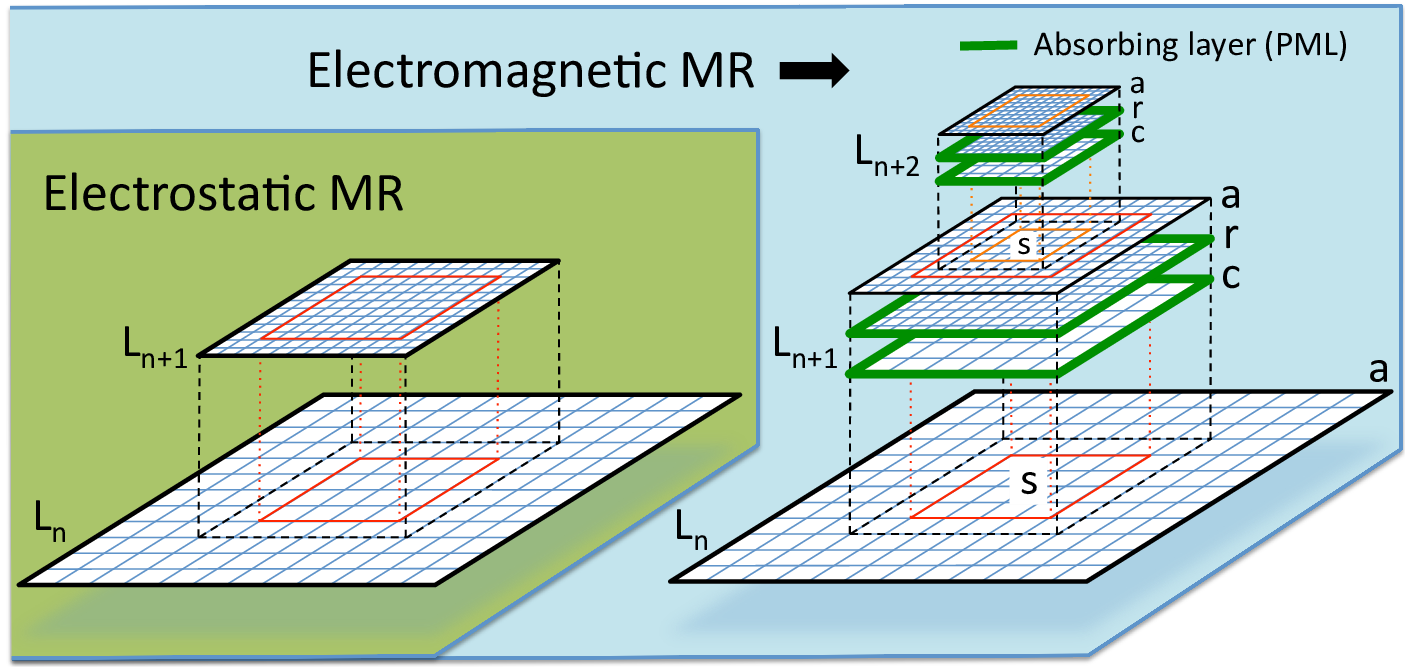
\includegraphics[width=15cm]{ICNSP_2011_Vay_fig1.png}
  \caption{Sketches of the implementation of mesh refinement in WarpX with the electrostatic (left) and electromagnetic (right) solvers. In both cases, the charge/current from particles are deposited at the finest levels first, then interpolated recursively to coarser levels. In the electrostatic case, the potential is calculated first at the coarsest level $L_0$, the solution interpolated to the boundaries of the refined patch $r$ at the next level $L_{1}$ and the potential calculated at $L_1$. The procedure is repeated iteratively up to the highest level.  In the electromagnetic case, the fields are computed independently on each grid and patch without interpolation at boundaries. Patches are terminated by absorbing layers (PML) to prevent the reflection of electromagnetic waves. Additional coarse patch $c$ and fine grid $a$ are needed so that the full solution is obtained by substitution on $a$ as $F_{n+1}(a)=F_{n+1}(r)+I[F_n( s )-F_{n+1}( c )]$ where $F$ is the field, and $I$ is a coarse-to-fine interpolation operator. In both cases, the field solution at a given level $L_n$ is unaffected by the solution at higher levels $L_{n+1}$ and up, allowing for mitigation of some spurious effects (see text) by providing a transition zone via extension of the patches by a few cells beyond the desired refined area (red \& orange rectangles) in which the field is interpolated onto particles from the coarser parent level only.}
  \label{fig:ESAMR}
\end{figure}

The mesh refinement methods that have been implemented in WarpX were developed following the following principles: i) avoidance of spurious effects from mesh refinement, or minimization of such effects; ii) user controllability of the spurious effects' relative magnitude; iii) simplicity of implementation. The two main generic issues that were identified are: a) spurious self-force on macroparticles close to the mesh refinement interface \cite{Vaylpb2002,Colellajcp2010}; b) reflection (and possible amplification) of short wavelength electromagnetic waves at the mesh refinement interface \cite{Vayjcp01}. The two effects are due to the loss of translation invariance introduced by the asymmetry of the grid on each side of the mesh refinement interface.

In addition, for some implementations where the field that is computed at a given level is affected by the solution at finer levels, there are cases where the procedure violates the integral of Gauss' Law around the refined patch, leading to long range errors \cite{Vaylpb2002,Colellajcp2010}. As will be shown below, in the procedure that has been developed in WarpX, the field at a given refinement level is not affected by the solution at finer levels, and is thus not affected by this type of error.

\subsection{Electrostatic}
A cornerstone of the Particle-In-Cell method is that assuming a particle lying in a hypothetical infinite grid, then if the grid is regular and symmetrical, and if the order of field gathering matches the order of charge (or current) deposition, then there is no self-force of the particle acting on itself: a) anywhere if using the so-called ``momentum conserving'' gathering scheme; b) on average within one cell if using the ``energy conserving'' gathering scheme \cite{Birdsalllangdon}. A breaking of the regularity and/or symmetry in the grid, whether it is from the use of irregular meshes or mesh refinement, and whether one uses finite difference, finite volume or finite elements, results in a net spurious self-force (which does not average to zero over one cell)  for a macroparticle close to the point of irregularity (mesh refinement interface for the current purpose) \cite{Vaylpb2002,Colellajcp2010}.

A sketch of the implementation of mesh refinement in WarpX is given in Figure~\ref{fig:ESAMR} (left). Given the solution of the electric potential at a refinement level $L_n$, it is interpolated onto the boundaries of the grid patch(es) at the next refined level $L_{n+1}$. The electric potential is then computed at level $L_{n+1}$ by solving the Poisson equation. This procedure necessitates the knowledge of the charge density at every level of refinement. For efficiency, the macroparticle charge is deposited on the highest level patch that contains them, and the charge density of each patch is added recursively to lower levels, down to the lowest.

\begin{figure}[htb]
  \centering
  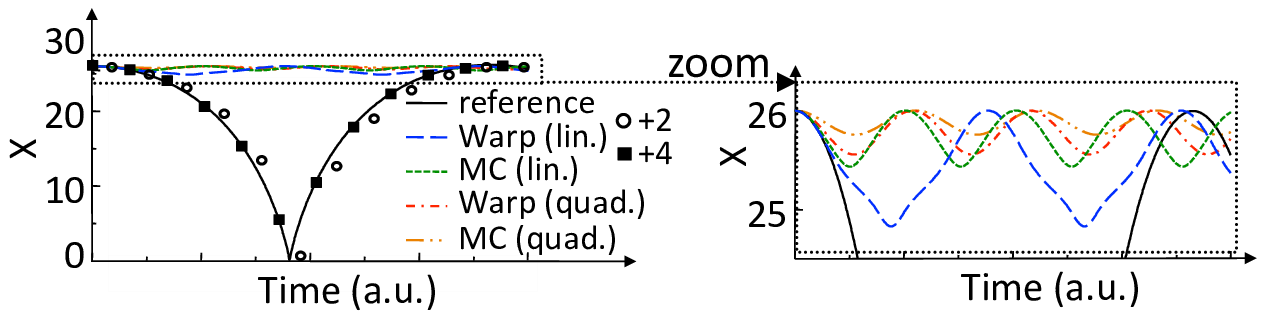
\includegraphics[width=15cm]{ICNSP_2011_Vay_fig2.png}
  \caption{Position history of one charged particle attracted by its image induced by a nearby metallic (dirichlet) boundary. The particle is initialized at rest. Without refinement patch (reference case), the particle is accelerated by its image, is reflected specularly at the wall, then decelerates until it reaches its initial position at rest. If the particle is initialized inside a refinement patch, the particle is initially accelerated toward the wall but is spuriously reflected before it reaches the boundary of the patch whether using the method implemented in WarpX or the MC method. Providing a surrounding transition region 2 or 4 cells wide in which the potential is interpolated from the parent coarse solution reduces significantly the effect of the spurious self-force. }
  \label{fig:ESselfforce}
\end{figure}
The presence of the self-force is illustrated on a simple test case that was introduced in \cite{Vaylpb2002} and also used in \cite{Colellajcp2010}: a single macroparticle is initialized at rest within a single refinement patch four cells away from the patch refinement boundary. The patch at level $L_1$ has $32\times32$ cells and is centered relative to the lowest $64\times64$ grid at level $L_0$ (``main grid''), while the macroparticle is centered in one direction but not in the other. The boundaries of the main grid are perfectly conducting, so that the macroparticle is attracted to the closest wall by its image. Specular reflection is applied when the particle reaches the boundary so that the motion is cyclic. The test was performed with WarpX using either linear or quadratic interpolation when gathering the main grid solution onto the refined patch boundary. It was also performed using another method from P. McCorquodale et al (labeled ``MC'' in this paper) based on the algorithm given in \cite{Mccorquodalejcp2004}, which employs a more elaborate procedure involving two-ways interpolations between the main grid and the refined patch. A reference case was also run using a single $128\times128$ grid with no refined patch, in which it is observed that the particle propagates toward the closest boundary at an accelerated pace, is reflected specularly at the boundary, then slows down until it reaches its initial position at zero velocity. The particle position histories are shown for the various cases in Fig. \ref{fig:ESselfforce}. In all the cases using the refinement patch, the particle was spuriously reflected near the patch boundary and was effectively trapped in the patch. We notice that linear interpolation performs better than quadratic, and that the simple method implemented in WarpX performs better than the other proposed method for this test (see discussion below).

\begin{figure}[htb]
  \centering
  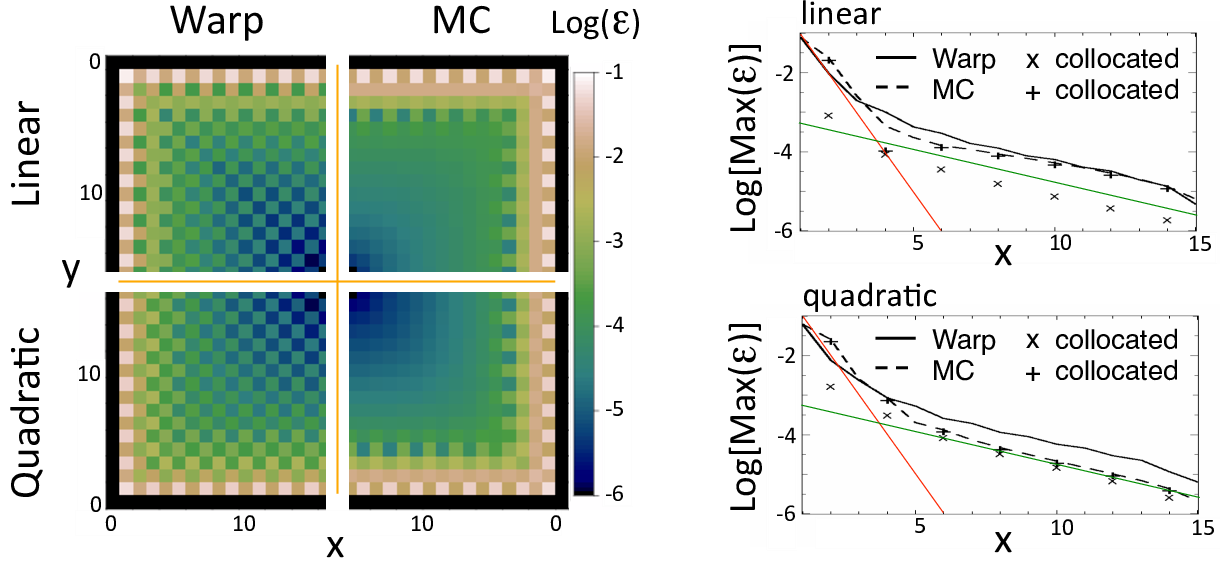
\includegraphics[width=15cm]{ICNSP_2011_Vay_fig3.png}
  \caption{(left) Maps of the magnitude of the spurious self-force $\epsilon$ in arbitrary units within one quarter of the refined patch, defined as $\epsilon=\sqrt{(E_x-E_x^{ref})^2+(E_y-E_y^{ref})^2}$, where $E_x$ and $E_y$ are the electric field components within the patch experienced by one particle at a given location and $E_x^{ref}$ and $E_y^{ref}$ are the electric field from a reference solution. The map is given for the WarpX and the MC mesh refinement algorithms and for linear and quadratic interpolation at the patch refinement boundary. \\(right) Lineouts of the maximum (taken over neighboring cells) of the spurious self-force. Close to the interface boundary (x=0), the spurious self-force decreases at a rate close to one order of magnitude per cell (red line), then at about one order of magnitude per six cells (green line).}
  \label{fig:ESselfforcemap}
\end{figure}
The magnitude of the spurious self-force as a function of the macroparticle position was mapped and is shown in Fig. \ref{fig:ESselfforcemap} for the WarpX and MC algorithms using linear or quadratic interpolations between grid levels. It is observed that the magnitude of the spurious self-force decreases rapidly with the distance between the particle and the refined patch boundary, at a rate approaching one order of magnitude per cell for the four cells closest to the boundary and about one order of magnitude per six cells beyond. The method implemented in WarpX offers a weaker spurious force on average and especially at the cells that are the closest to the coarse-fine interface where it is the largest and thus matters most.
We notice that the magnitude of the spurious self-force depends strongly on the distance to the edge of the patch and to the nodes of the underlying coarse grid, but weakly on the order of deposition and size of the patch.

A method was devised and implemented in WarpX for reducing the magnitude of spurious self-forces near the coarse-fine boundaries as follows. Noting that the coarse grid solution is unaffected by the presence of the patch and is thus free of self-force, extra ``transition'' cells  are added around the ``effective'' refined area.
Within the effective area, the particles gather the potential in the fine grid. In the extra transition cells surrounding the refinement patch, the force is gathered directly from the coarse grid (an option, which has not yet been implemented, would be to interpolate between the coarse and fine grid field solutions within the transition zone so as to provide continuity of the force experienced by the particles at the interface). The number of cells allocated in the transition zones is controllable by the user in WarpX, giving the opportunity to check whether the spurious self-force is affecting the calculation by repeating it using different thicknesses of the transition zones. The control of the spurious force using the transition zone is illustrated in Fig.~\ref{fig:ESselfforce}, where the calculation with WarpX using linear interpolation at the patch interface was repeated using either two or four cells transition regions (measured in refined patch cell units). Using two extra cells allowed for the particle to be free of spurious trapping within the refined area and follow a trajectory that is close to the reference one, and using four extra cells improved further to the point where the resulting trajectory becomes undistinguishable from the reference one.
We note that an alternative method was devised for reducing the magnitude of self-force near the coarse-fine boundaries for the MC method, by using a special deposition procedure near the interface \cite{Colellajcp2010}.

%\begin{figure}[htb]
%  \centering
%  \includegraphics[width=15cm]{ICNSP_2011_Vay_fig4.png}
%  \caption{Snapshot from a 3D self-consistent simulation of the injector in the High Current Experiment shows the beam emerging from the source at low energy (blue) and being accelerated (green-yellow-orange) and transported in a four quadrupole front end. The automatic layout of the mesh refinement patches from a 2D axisymmetric simulation of the source area shows 2 levels of refinement, concentrating the finer meshes around the emitter (white curve surface) and the beam edge (dark blue).}
%  \label{fig:ESHCX}
%\end{figure}
%Automatic remeshing has been implemented in WarpX following the procedure described in \cite{Vaynim2005}, refining on criteria based on measures of local charge density magnitude and gradients. AMR WarpX simulations were applied to the modeling of the front end injector of the High Current Experiment (HCX) \cite{Prostprstab2005}, and provided the first numerically converged estimates of phase space beam distorsions, which directly affects beam quality \cite{Vaypop04}. Fig.~\ref{fig:ESHCX} shows snapshots from 2D axisymmetric simulation of the souce area illustrating the automatic placement of refined patches, and 3D simulation of the full injector showing the beam generation, acceleration and transport.

\subsection{Electromagnetic}
The method that is used for electrostatic mesh refinement is not directly applicable to electromagnetic calculations. As was shown in section 3.4 of \cite{Vayjcp01}, refinement schemes relying solely on interpolation between coarse and fine patches lead to the reflection with amplification of the short wavelength modes that fall below the cutoff of the Nyquist frequency of the coarse grid. Unless these modes are damped heavily or prevented from occurring at their source, they may affect particle motion and their effect can escalate if trapped within a patch, via multiple successive reflections with amplification.

To circumvent this issue, an additional coarse patch (with the same resolution as the parent grid) is added, as shown in Fig.~\ref{fig:ESAMR}-right and described in \cite{Vaycpc04}. Both the fine and the coarse grid patches are terminated by Perfectly Matched Layers, reducing wave reflection by orders of magnitude, controllable by the user \cite{Berengerjcp96,Vayjcp02}. The source current resulting from the motion of charged macroparticles within the refined region is accumulated on the fine patch and is then interpolated onto the coarse patch and added onto the parent grid. The process is repeated recursively from the finest level down to the coarsest. The Maxwell equations are then solved for one time interval on the entire set of grids, by default for one time step using the time step of the finest grid. The field on the coarse and fine patches only contain the contributions from the particles that have evolved within the refined area but not from the current sources outside the area. The total contribution of the field from sources within and outside the refined area is obtained by adding the field from the refined grid $F(r)$, and adding an interpolation $I$ of the difference between the relevant subset $s$ of the field in the parent grid $F(s)$ and the field of the coarse grid  $F( c )$, on an auxiliary grid $a$, i.e. $F(a)=F(r)+I[F(s)-F( c )]$. The field on the parent grid subset $F(s)$ contains contributions from sources from both within and outside of the refined area. Thus, in effect, there is substitution of the coarse field resulting from sources within the patch area by its fine resolution counterpart. The operation is carried out recursively starting at the coarsest level up to the finest.
An option has been implemented in which various grid levels are pushed with different time steps, given as a fixed fraction of the individual grid Courant conditions (assuming same cell aspect ratio for all grids and refinement by integer factors). In this case, the fields from the coarse levels, which are advanced less often, are interpolated in time.

The substitution method has two potential drawbacks due to the inexact cancellation between the coarse and fine patches of : (i) the remnants of ghost fixed charges created by the particles entering and leaving the patches (this effect is due to the use of the electromagnetic solver and is different from the spurious self-force that was described for the electrostatic case); (ii) if using a Maxwell solver with a low-order stencil, the electromagnetic waves traveling on each patch at slightly different velocity due to numerical dispersion.
The first issue results in an effective spurious multipole field whose magnitude decreases very rapidly with the distance to the patch boundary, similarly to the spurious self-force in the electrostatic case. Hence, adding a few extra transition cells surrounding the patches mitigates this effect very effectively.
%[Add hyperbolic correction?]
The tunability of WarpX's electromagnetic finite-difference and pseudo-spectral solvers provides the means to optimize the numerical dispersion so as to minimize the second effect for a given application, which has been demonstrated on the laser-plasma interaction test case presented in \cite{Vaycpc04}.
Both effects and their mitigation are described in more detail in \cite{Vaycpc04}.

Caustics are supported anywhere on the grid with an accuracy that is set by the local resolution, and will be adequately resolved if the grid resolution supports the necessary  modes from their sources to the points of wavefront crossing. The mesh refinement method that is implemented in WarpX has the potential to provide higher efficiency than the standard use of fixed gridding, by offering a path toward adaptive gridding following wavefronts.

%\begin{figure}[htb]
%  \centering
%  \includegraphics[width=13cm]{ICNSP_2011_Vay_fig5.png}
%  \caption{Electron density $n_e$ (normalized to the density of the injected plasma) from WarpX simulations  in 2-1/2D for a), b), c) and 3D for d) of a rigid beam (thin light-blue outline) propagating through a neutral plasma, for grid sizes of a) $128\times320$, b) $512\times1280$, c) $128\times320$ (main grid, red box) + $128\times640$ (patch 1, orange box) + $128\times1280$ (patch 2, yellow box), such that the resolution of patch 2 matched the resolution of the grid used for b), d) grid size of $64\times64\times160$ (main grid, red box) + $64\times64\times320$ (patch 1, orange box) + $64\times64\times640$ (patch 2, yellow box). For c) and d),  the number and weight of injected plasma macroparticles was adjusted to keep the number of macroparticles per cell constant in each grid at injection in front of the beam.}
%  \label{fig:EMplasma}
%\end{figure}
%As a test to the electromagnetic PIC implementation, WarpX simulations of wave excitations by a beam propagating through plasma, as described in \cite{Kaganovichpop2004}, were conducted. In these simulations, a hard-edged, elliptical, rigid beam propagates at constant velocity $v_z = 0.5c$ where $c$ is the speed of light through an initially cold neutral plasma of initial density $n_0$. The beam has a flat-top density profile of $n_b = n_0/2$, and an elliptical shape of length $l = 15 c/\omega_p$ and diameter $d = l/10$, where $\omega_p$ is the electron plasma frequency. It is shown in  \cite{Kaganovichpop2004} that waves with a wavenumber of approximately $2\omega_p/v_z$ are generated in the plasma by the beam's electrostatic field, and have larger amplitude inside the beam, due to their interaction with the beam's sharp edges.

%Resolving the beam edge and the small structures developing in the wake inside the beam forces small cell sizes. The resolution that is needed for macroscopic convergence was explored in 2-1/2D in a series of four runs where the number of grid cells was varied from $64\times160$ to $512\times1280$ by incremental factors of 2. Third order spline interpolation was used for the beam and plasma macroparticle current deposition and force gathering. The details of the plasma wake were very similar between the two highest resolution cases, indicating that macroscopic convergence was reached. The results from the runs using $128\times320$ and $512\times1280$ grids are shown in Fig.~\ref{fig:EMplasma}. The result from the highest resolution run serves as the reference for subsequent calculations with mesh refinement.

%A run was conducted where the main grid had $128\times320$ cells and was complemented by two refinement patches (with successive refinement factors of 2 in each direction), such that the resolution in the central patch matched the resolution of the case of reference.
%The number and weight of the injected plasma macroparticles was varied, such that the number of macroparticles per cell in each grid at injection was constant. Results are plotted in Fig.~\ref{fig:EMplasma} (bottom-left) showing a good reproduction of the fine scale structures within the central fine patch in good agreement with the reference case.
%Lastly, a three-dimensional simulation with mesh refinement of the same physical setup was conducted. The grid setup and 3D isosurfaces of the plasma electron density as the beam enters the plasma are shown in Fig.~\ref{fig:EMplasma} (bottom-right). As expected, structures similar to the ones observed in 2D are present within the beam envelope. The speedup achieved by the use of mesh refinement was estimated to be approximately one order of magnitude in 3D.


%%%%%% Copyright 2017-2019 Jean-Luc Vay, Remi Lehe
%
% This file is part of WarpX.
%
% License: BSD-3-Clause-LBNL


\usepackage{bm}
\usepackage{amsmath}
\usepackage{amssymb}
\usepackage{graphicx}
\usepackage{url}
\usepackage{hyperref}

\usepackage[displaymath]{lineno}\usepackage{bm}% bold math

\newcommand{\fe}{\mathbf{\tilde{E}}}
\newcommand{\fb}{\mathbf{\tilde{B}}}
\newcommand{\fj}{\mathbf{\tilde{J}}}
\newcommand{\ff}{\tilde{F}}
\newcommand{\fg}{\tilde{G}}
\newcommand{\fk}{\mathbf{k}}
\newcommand{\fkhat}{\mathbf{\hat{k}}}

% Definitions from Remi's paper on Galilean math
\newcommand{\Km}{\vec{K}_{\vec{m}}}
\newcommand{\km}{\vec{k}_{\vec{m}}}
\renewcommand{\vec}[1]{\boldsymbol{#1}}
\newcommand{\vgal}{\vec{v}_{gal}}
\newcommand{\nab}{\vec{\nabla'}}
\newcommand{\Dt}[1]{ \frac{\partial #1}{\partial t}}
\newcommand{\mc}[1]{\hat{\mathcal{#1}}}
\newcommand{\xj}{\vec{x}'_{\vec{j}}}
\newcommand{\Xll}{\vec{X}_{\vec{\ell}}}
\newcommand{\Integ}[1]{\int_{-\infty}^{\infty} \!\!\!\!\!\!
  \mathrm{d}#1}
\newcommand{\RInteg}[1]{\int_{0}^{\infty} \!\! \frac{#1\mathrm{d}#1}{(2\pi)^2}}

% Definitions from Remi's Thesis
\newcommand{\h}{\mathcal{H}}
\newcommand{\hf}{\frac{1}{2}}
\newcommand{\um}{$\mu$m}
\newcommand{\Um}{\mu \mathrm{m}}
\newcommand{\aal}{\langle \vec{a}_l^2 \rangle}
\newcommand{\etad}{ \eta_d }
\newcommand{\etae}{ \eta_\epsilon }
\newcommand{\etag}{ \eta_\gamma }
\newcommand{\tlambda}{ \tilde{\lambda} }
%\newcommand\comment[1]{\textcolor{red}{\textbf{#1}}}
\newcommand{\gsim}{\mathrel{\hbox{\rlap{\lower.55ex
\hbox{$\sim$}} \kern-.3em \raise.4ex \hbox{$>$}}}}
\newcommand{\lsim}{\mathrel{\hbox{\rlap{\lower.55ex
\hbox{$\sim$}} \kern-.3em \raise.4ex \hbox{$<$}}}}
\newcommand{\kfoc}{k_\mathrm{foc}}
\newcommand{\bkfoc}{\bar{k}_\mathrm{foc}}
\newcommand{\xil}{\xi_{\mathrm{laser}}}

\newcommand{\Ex}[2]{{E_x}^{#1}_{#2}}
\newcommand{\Ey}[2]{{E_y}^{#1}_{#2}}
\newcommand{\Ez}[2]{{E_z}^{#1}_{#2}}
\newcommand{\Bx}[2]{{B_x}^{#1}_{#2}}
\newcommand{\By}[2]{{B_y}^{#1}_{#2}}
\newcommand{\Bz}[2]{{B_z}^{#1}_{#2}}
\newcommand{\Jx}[2]{{J_x}^{#1}_{#2}}
\newcommand{\Jy}[2]{{J_y}^{#1}_{#2}}
\newcommand{\Jz}[2]{{J_z}^{#1}_{#2}}

\newcommand{\tEr}[2]{\tilde{E_r}^{#1}_{#2}}
\newcommand{\tEt}[2]{\tilde{E_\theta}^{#1}_{#2}}
\newcommand{\tEz}[2]{\tilde{E_z}^{#1}_{#2}}
\newcommand{\tBr}[2]{\tilde{B_r}^{#1}_{#2}}
\newcommand{\tBt}[2]{\tilde{B_\theta}^{#1}_{#2}}
\newcommand{\tBz}[2]{\tilde{B_z}^{#1}_{#2}}
\newcommand{\tJr}[2]{\tilde{J_r}^{#1}_{#2}}
\newcommand{\tJt}[2]{\tilde{J_\theta}^{#1}_{#2}}
\newcommand{\tJz}[2]{\tilde{J_z}^{#1}_{#2}}

\newcommand{\CCirc}{\textsc{Calder Circ}}
\newcommand{\CCart}{\textsc{Calder 3D}}

It was shown in \cite{VayPOP2008} that the Boris formulation is
not Lorentz invariant and can lead to significant errors in the treatment
of relativistic dynamics. A Lorentz invariant formulation is obtained
by considering the following velocity average 
\begin{align}
\mathbf{\bar{v}}^{i}= & \frac{\mathbf{v}^{i+1/2}+\mathbf{v}^{i-1/2}}{2},\label{Eq:new_v}
\end{align}
This gives a system that is solvable analytically (see \cite{VayPOP2008}
for a detailed derivation), giving the following velocity update:

\begin{subequations}
\begin{align}
\mathbf{u^{*}}= & \mathbf{u}^{i-1/2}+\frac{q\Delta t}{m}\left(\mathbf{E}^{i}+\frac{\mathbf{v}^{i-1/2}}{2}\times\mathbf{B}^{i}\right),\label{pusher_gamma}\\
\mathbf{u}^{i+1/2}= & \left[\mathbf{u^{*}}+\left(\mathbf{u^{*}}\cdot\mathbf{t}\right)\mathbf{t}+\mathbf{u^{*}}\times\mathbf{t}\right]/\left(1+t^{2}\right),\label{pusher_upr}
\end{align}
\end{subequations}
where $\mathbf{t}=\bm{\tau}/\gamma^{i+1/2}$, $\bm{\tau}=\left(q\Delta t/2m\right)\mathbf{B}^{i}$,
$\gamma^{i+1/2}=\sqrt{\sigma+\sqrt{\sigma^{2}+\left(\tau^{2}+w^{2}\right)}}$,
$w=\mathbf{u^{*}}\cdot\bm{\tau}$, $\sigma=\left(\gamma'^{2}-\tau^{2}\right)/2$
and $\gamma'=\sqrt{1+(\mathbf{u}^{*}/c)^{2}}$. This Lorentz invariant formulation
is particularly well suited for the modeling of ultra-relativistic
charged particle beams, where the accurate account of the cancellation
of the self-generated electric and magnetic fields is essential, as
shown in \cite{VayPOP2008}.

%%%%%%%%%%%%%%%%%%%%%%%%%%%%%%
\section{Boundary conditions}
%%%%%%%%%%%%%%%%%%%%%%%%%%%%%%%%%%%
% Copyright 2017-2019 Jean-Luc Vay, Remi Lehe
%
% This file is part of WarpX.
%
% License: BSD-3-Clause-LBNL


\usepackage{bm}
\usepackage{amsmath}
\usepackage{amssymb}
\usepackage{graphicx}
\usepackage{url}
\usepackage{hyperref}

\usepackage[displaymath]{lineno}\usepackage{bm}% bold math

\newcommand{\fe}{\mathbf{\tilde{E}}}
\newcommand{\fb}{\mathbf{\tilde{B}}}
\newcommand{\fj}{\mathbf{\tilde{J}}}
\newcommand{\ff}{\tilde{F}}
\newcommand{\fg}{\tilde{G}}
\newcommand{\fk}{\mathbf{k}}
\newcommand{\fkhat}{\mathbf{\hat{k}}}

% Definitions from Remi's paper on Galilean math
\newcommand{\Km}{\vec{K}_{\vec{m}}}
\newcommand{\km}{\vec{k}_{\vec{m}}}
\renewcommand{\vec}[1]{\boldsymbol{#1}}
\newcommand{\vgal}{\vec{v}_{gal}}
\newcommand{\nab}{\vec{\nabla'}}
\newcommand{\Dt}[1]{ \frac{\partial #1}{\partial t}}
\newcommand{\mc}[1]{\hat{\mathcal{#1}}}
\newcommand{\xj}{\vec{x}'_{\vec{j}}}
\newcommand{\Xll}{\vec{X}_{\vec{\ell}}}
\newcommand{\Integ}[1]{\int_{-\infty}^{\infty} \!\!\!\!\!\!
  \mathrm{d}#1}
\newcommand{\RInteg}[1]{\int_{0}^{\infty} \!\! \frac{#1\mathrm{d}#1}{(2\pi)^2}}

% Definitions from Remi's Thesis
\newcommand{\h}{\mathcal{H}}
\newcommand{\hf}{\frac{1}{2}}
\newcommand{\um}{$\mu$m}
\newcommand{\Um}{\mu \mathrm{m}}
\newcommand{\aal}{\langle \vec{a}_l^2 \rangle}
\newcommand{\etad}{ \eta_d }
\newcommand{\etae}{ \eta_\epsilon }
\newcommand{\etag}{ \eta_\gamma }
\newcommand{\tlambda}{ \tilde{\lambda} }
%\newcommand\comment[1]{\textcolor{red}{\textbf{#1}}}
\newcommand{\gsim}{\mathrel{\hbox{\rlap{\lower.55ex
\hbox{$\sim$}} \kern-.3em \raise.4ex \hbox{$>$}}}}
\newcommand{\lsim}{\mathrel{\hbox{\rlap{\lower.55ex
\hbox{$\sim$}} \kern-.3em \raise.4ex \hbox{$<$}}}}
\newcommand{\kfoc}{k_\mathrm{foc}}
\newcommand{\bkfoc}{\bar{k}_\mathrm{foc}}
\newcommand{\xil}{\xi_{\mathrm{laser}}}

\newcommand{\Ex}[2]{{E_x}^{#1}_{#2}}
\newcommand{\Ey}[2]{{E_y}^{#1}_{#2}}
\newcommand{\Ez}[2]{{E_z}^{#1}_{#2}}
\newcommand{\Bx}[2]{{B_x}^{#1}_{#2}}
\newcommand{\By}[2]{{B_y}^{#1}_{#2}}
\newcommand{\Bz}[2]{{B_z}^{#1}_{#2}}
\newcommand{\Jx}[2]{{J_x}^{#1}_{#2}}
\newcommand{\Jy}[2]{{J_y}^{#1}_{#2}}
\newcommand{\Jz}[2]{{J_z}^{#1}_{#2}}

\newcommand{\tEr}[2]{\tilde{E_r}^{#1}_{#2}}
\newcommand{\tEt}[2]{\tilde{E_\theta}^{#1}_{#2}}
\newcommand{\tEz}[2]{\tilde{E_z}^{#1}_{#2}}
\newcommand{\tBr}[2]{\tilde{B_r}^{#1}_{#2}}
\newcommand{\tBt}[2]{\tilde{B_\theta}^{#1}_{#2}}
\newcommand{\tBz}[2]{\tilde{B_z}^{#1}_{#2}}
\newcommand{\tJr}[2]{\tilde{J_r}^{#1}_{#2}}
\newcommand{\tJt}[2]{\tilde{J_\theta}^{#1}_{#2}}
\newcommand{\tJz}[2]{\tilde{J_z}^{#1}_{#2}}

\newcommand{\CCirc}{\textsc{Calder Circ}}
\newcommand{\CCart}{\textsc{Calder 3D}}

\subsection{Open boundary condition for electromagnetic waves}

For the TE case, the original Berenger's Perfectly Matched Layer (PML) writes

% PML
\begin{eqnarray}
\varepsilon _{0}\frac{\partial E_{x}}{\partial t}+\sigma _{y}E_{x} = & \frac{\partial H_{z}}{\partial y}\label{PML_def_1} \\
\varepsilon _{0}\frac{\partial E_{y}}{\partial t}+\sigma _{x}E_{y} = & -\frac{\partial H_{z}}{\partial x}\label{PML_def_2} \\
\mu _{0}\frac{\partial H_{zx}}{\partial t}+\sigma ^{*}_{x}H_{zx} = & -\frac{\partial E_{y}}{\partial x}\label{PML_def_3} \\
\mu _{0}\frac{\partial H_{zy}}{\partial t}+\sigma ^{*}_{y}H_{zy} = & \frac{\partial E_{x}}{\partial y}\label{PML_def_4} \\
H_{z}  = & H_{zx}+H_{zy}\label{PML_def_5} 
\end{eqnarray}

This can be generalized to

% APML
\begin{eqnarray}
\varepsilon _{0}\frac{\partial E_{x}}{\partial t}+\sigma _{y}E_{x} = & \frac{c_{y}}{c}\frac{\partial H_{z}}{\partial y}+\overline{\sigma }_{y}H_{z}\label{APML_def_1} \\
\varepsilon _{0}\frac{\partial E_{y}}{\partial t}+\sigma _{x}E_{y} = & -\frac{c_{x}}{c}\frac{\partial H_{z}}{\partial x}+\overline{\sigma }_{x}H_{z}\label{APML_def_2} \\
\mu _{0}\frac{\partial H_{zx}}{\partial t}+\sigma ^{*}_{x}H_{zx} = & -\frac{c^{*}_{x}}{c}\frac{\partial E_{y}}{\partial x}+\overline{\sigma }_{x}^{*}E_{y}\label{APML_def_3} \\
\mu _{0}\frac{\partial H_{zy}}{\partial t}+\sigma ^{*}_{y}H_{zy} = & \frac{c^{*}_{y}}{c}\frac{\partial E_{x}}{\partial y}+\overline{\sigma }_{y}^{*}E_{x}\label{APML_def_4} \\
H_{z} = & H_{zx}+H_{zy}\label{APML_def_5} 
\end{eqnarray}

For $c_{x}=c_{y}=c^{*}_{x}=c^{*}_{y}=c$ and $\overline{\sigma }_{x}=\overline{\sigma }_{y}=\overline{\sigma }_{x}^{*}=\overline{\sigma }_{y}^{*}=0$,
this system reduces to the Berenger PML medium, while adding the additional
constraint $\sigma _{x}=\sigma _{y}=\sigma _{x}^{*}=\sigma _{y}^{*}=0$
leads to the system of Maxwell equations in vacuum.

\subsubsection{\label{Sec:analytic theory, propa plane wave}Propagation of a Plane Wave in an APML Medium}

We consider a plane wave of magnitude ($ E_{0},H_{zx0},H_{zy0} $)
and pulsation $\omega$ propagating in the APML medium with an
angle $\varphi$ relative to the x axis

\begin{eqnarray}
E_{x} = & -E_{0}\sin \varphi e^{i\omega \left( t-\alpha x-\beta y\right) }\label{Plane_wave_APML_def_1} \\
E_{y} = & E_{0}\cos \varphi e^{i\omega \left( t-\alpha x-\beta y\right) }\label{Plane_wave_APML_def_2} \\
H_{zx} = & H_{zx0}e^{i\omega \left( t-\alpha x-\beta y\right) }\label{Plane_wave_AMPL_def_3} \\
H_{zy} = & H_{zy0}e^{i\omega \left( t-\alpha x-\beta y\right) }\label{Plane_wave_APML_def_4} 
\end{eqnarray}


where $\alpha$ and$\beta$ are two complex constants to
be determined.

Introducing (\ref{Plane_wave_APML_def_1}), (\ref{Plane_wave_APML_def_2}),
(\ref{Plane_wave_AMPL_def_3}) and (\ref{Plane_wave_APML_def_4})
into (\ref{APML_def_1}), (\ref{APML_def_2}), (\ref{APML_def_3})
and (\ref{APML_def_4}) gives

\begin{eqnarray}
\varepsilon _{0}E_{0}\sin \varphi -i\frac{\sigma _{y}}{\omega }E_{0}\sin \varphi  = & \beta \frac{c_{y}}{c}\left( H_{zx0}+H_{zy0}\right) +i\frac{\overline{\sigma }_{y}}{\omega }\left( H_{zx0}+H_{zy0}\right) \label{Plane_wave_APML_1_1} \\
\varepsilon _{0}E_{0}\cos \varphi -i\frac{\sigma _{x}}{\omega }E_{0}\cos \varphi  = & \alpha \frac{c_{x}}{c}\left( H_{zx0}+H_{zy0}\right) -i\frac{\overline{\sigma }_{x}}{\omega }\left( H_{zx0}+H_{zy0}\right) \label{Plane_wave_APML_1_2} \\
\mu _{0}H_{zx0}-i\frac{\sigma ^{*}_{x}}{\omega }H_{zx0} = & \alpha \frac{c^{*}_{x}}{c}E_{0}\cos \varphi -i\frac{\overline{\sigma }^{*}_{x}}{\omega }E_{0}\cos \varphi \label{Plane_wave_APML_1_3} \\
\mu _{0}H_{zy0}-i\frac{\sigma ^{*}_{y}}{\omega }H_{zy0} = & \beta \frac{c^{*}_{y}}{c}E_{0}\sin \varphi +i\frac{\overline{\sigma }^{*}_{y}}{\omega }E_{0}\sin \varphi \label{Plane_wave_APML_1_4} 
\end{eqnarray}


Defining $Z=E_{0}/\left( H_{zx0}+H_{zy0}\right)$ and using (\ref{Plane_wave_APML_1_1})
and (\ref{Plane_wave_APML_1_2}), we get

\begin{eqnarray}
\beta  = & \left[ Z\left( \varepsilon _{0}-i\frac{\sigma _{y}}{\omega }\right) \sin \varphi -i\frac{\overline{\sigma }_{y}}{\omega }\right] \frac{c}{c_{y}}\label{Plane_wave_APML_beta_of_g} \\
\alpha  = & \left[ Z\left( \varepsilon _{0}-i\frac{\sigma _{x}}{\omega }\right) \cos \varphi +i\frac{\overline{\sigma }_{x}}{\omega }\right] \frac{c}{c_{x}}\label{Plane_wave_APML_alpha_of_g} 
\end{eqnarray}


Adding $H_{zx0}$ and $H_{zy0}$ from (\ref{Plane_wave_APML_1_3})
and (\ref{Plane_wave_APML_1_4}) and substituting the expressions
for $\alpha$ and $\beta$ from (\ref{Plane_wave_APML_beta_of_g})
and (\ref{Plane_wave_APML_alpha_of_g}) yields

\begin{eqnarray}
\frac{1}{Z} = & \frac{Z\left( \varepsilon _{0}-i\frac{\sigma _{x}}{\omega }\right) \cos \varphi \frac{c^{*}_{x}}{c_{x}}+i\frac{\overline{\sigma }_{x}}{\omega }\frac{c^{*}_{x}}{c_{x}}-i\frac{\overline{\sigma }^{*}_{x}}{\omega }}{\mu _{0}-i\frac{\sigma ^{*}_{x}}{\omega }}\cos \varphi \nonumber \\
 + & \frac{Z\left( \varepsilon _{0}-i\frac{\sigma _{y}}{\omega }\right) \sin \varphi \frac{c^{*}_{y}}{c_{y}}-i\frac{\overline{\sigma }_{y}}{\omega }\frac{c^{*}_{y}}{c_{y}}+i\frac{\overline{\sigma }^{*}_{y}}{\omega }}{\mu _{0}-i\frac{\sigma ^{*}_{y}}{\omega }}\sin \varphi 
\end{eqnarray}


If $c_{x}=c^{*}_{x}$, $c_{y}=c^{*}_{y}$, $\overline{\sigma }_{x}=\overline{\sigma }^{*}_{x}$, $\overline{\sigma }_{y}=\overline{\sigma }^{*}_{y}$, $\frac{\sigma _{x}}{\varepsilon _{0}}=\frac{\sigma ^{*}_{x}}{\mu _{0}}$ and $\frac{\sigma _{y}}{\varepsilon _{0}}=\frac{\sigma ^{*}_{y}}{\mu _{0}}$ then

\begin{eqnarray}
Z = & \pm \sqrt{\frac{\mu _{0}}{\varepsilon _{0}}}\label{APML_impedance} 
\end{eqnarray}


which is the impedance of vacuum. Hence, like the PML, given some
restrictions on the parameters, the APML does not generate any reflection
at any angle and any frequency. As for the PML, this property is not
retained after discretization, as shown subsequently in this paper.

Calling $\psi$ any component of the field and $\psi _{0}$
its magnitude, we get from (\ref{Plane_wave_APML_def_1}), (\ref{Plane_wave_APML_beta_of_g}),
(\ref{Plane_wave_APML_alpha_of_g}) and (\ref{APML_impedance}) that 

\begin{equation}
\label{Plane_wave_absorption}
\psi =\psi _{0}e^{i\omega \left( t\mp x\cos \varphi /c_{x}\mp y\sin \varphi /c_{y}\right) }e^{-\left( \pm \frac{\sigma _{x}\cos \varphi }{\varepsilon _{0}c_{x}}+\overline{\sigma }_{x}\frac{c}{c_{x}}\right) x}e^{-\left( \pm \frac{\sigma _{y}\sin \varphi }{\varepsilon _{0}c_{y}}+\overline{\sigma }_{y}\frac{c}{c_{y}}\right) y}
\end{equation}


We assume that we have an APML layer of thickness $\delta$ (measured
along $x$) and that $\sigma _{y}=\overline{\sigma }_{y}=0$
and $c_{y}=c.$ Using (\ref{Plane_wave_absorption}), we determine
that the coefficient of reflection given by this layer is 

\begin{eqnarray}
R_{APML}\left( \theta \right)  = & e^{-\left( \sigma _{x}\cos \varphi /\varepsilon _{0}c_{x}+\overline{\sigma }_{x}c/c_{x}\right) \delta }e^{-\left( \sigma _{x}\cos \varphi /\varepsilon _{0}c_{x}-\overline{\sigma }_{x}c/c_{x}\right) \delta }\nonumber \\
 = & e^{-2\left( \sigma _{x}\cos \varphi /\varepsilon _{0}c_{x}\right) \delta }
\end{eqnarray}


which happens to be the same as the PML theoretical coefficient of
reflection if we assume $c_{x}=c$. Hence, it follows that for
the purpose of wave absorption, the term $\overline{\sigma }_{x}$
seems to be of no interest. However, although this conclusion is true
at the infinitesimal limit, it does not hold for the discretized counterpart.

\subsubsection{Discretization}

%
\begin{subequations}
\begin{align}
\frac{E_x|^{n+1}_{j+1/2,k,l}-E_x|^{n}_{j+1/2,k,l}}{\Delta t} + \sigma_y \frac{E_x|^{n+1}_{j+1/2,k,l}+E_x|^{n}_{j+1/2,k,l}}{2} = & \frac{H_z|^{n+1/2}_{j+1/2,k+1/2,l}-H_z|^{n+1/2}_{j+1/2,k-1/2,l}}{\Delta y} \\
%
\frac{E_y|^{n+1}_{j,k+1/2,l}-E_y|^{n}_{j,k+1/2,l}}{\Delta t} + \sigma_x \frac{E_y|^{n+1}_{j,k+1/2,l}+E_y|^{n}_{j,k+1/2,l}}{2} = & - \frac{H_z|^{n+1/2}_{j+1/2,k+1/2,l}-H_z|^{n+1/2}_{j-1/2,k+1/2,l}}{\Delta x} \\
%
\frac{H_{zx}|^{n+3/2}_{j+1/2,k+1/2,l}-H_{zx}|^{n}_{j+1/2,k+1/2,l}}{\Delta t} + \sigma^*_x \frac{H_{zx}|^{n+3/2}_{j+1/2,k+1/2,l}+H_{zx}|^{n}_{j+1/2,k+1/2,l}}{2} = & - \frac{E_y|^{n+1}_{j+1,k+1/2,l}-E_y|^{n+1}_{j,k+1/2,l}}{\Delta x} \\
%
\frac{H_{zy}|^{n+3/2}_{j+1/2,k+1/2,l}-H_{zy}|^{n}_{j+1/2,k+1/2,l}}{\Delta t} + \sigma^*_y \frac{H_{zy}|^{n+3/2}_{j+1/2,k+1/2,l}+H_{zy}|^{n}_{j+1/2,k+1/2,l}}{2} = & \frac{E_x|^{n+1}_{j+1/2,k+1,l}-E_x|^{n+1}_{j+1/2,k,l}}{\Delta y} \\
%
H_z = & H_{zx}+H_{zy}
\end{align}
\end{subequations}

%
\begin{subequations}
\begin{align}
E_x|^{n+1}_{j+1/2,k,l} = & \left(\frac{1-\sigma_y \Delta t/2}{1+\sigma_y \Delta t/2}\right) E_x|^{n}_{j+1/2,k,l} + \frac{\Delta t/\Delta y}{1+\sigma_y \Delta t/2} \left(H_z|^{n+1/2}_{j+1/2,k+1/2,l}-H_z|^{n+1/2}_{j+1/2,k-1/2,l}\right) \\
%
E_y|^{n+1}_{j,k+1/2,l} = & \left(\frac{1-\sigma_x \Delta t/2}{1+\sigma_x \Delta t/2}\right) E_y|^{n}_{j,k+1/2,l} - \frac{\Delta t/\Delta x}{1+\sigma_x \Delta t/2} \left(H_z|^{n+1/2}_{j+1/2,k+1/2,l}-H_z|^{n+1/2}_{j-1/2,k+1/2,l}\right) \\
%
H_{zx}|^{n+3/2}_{j+1/2,k+1/2,l} = & \left(\frac{1-\sigma^*_x \Delta t/2}{1+\sigma^*_x \Delta t/2}\right) H_{zx}|^{n}_{j+1/2,k+1/2,l} - \frac{\Delta t/\Delta x}{1+\sigma^*_x \Delta t/2} \left(E_y|^{n+1}_{j+1,k+1/2,l}-E_y|^{n+1}_{j,k+1/2,l}\right) \\
%
H_{zy}|^{n+3/2}_{j+1/2,k+1/2,l} = & \left(\frac{1-\sigma^*_y \Delta t/2}{1+\sigma^*_y \Delta t/2}\right) H_{zy}|^{n}_{j+1/2,k+1/2,l} + \frac{\Delta t/\Delta y}{1+\sigma^*_y \Delta t/2} \left(E_x|^{n+1}_{j+1/2,k+1,l}-E_x|^{n+1}_{j+1/2,k,l}\right) \\
%
H_z = & H_{zx}+H_{zy}
\end{align}
\end{subequations}

%
\begin{subequations}
\begin{align}
E_x|^{n+1}_{j+1/2,k,l} = & E_x|^{n}_{j+1/2,k,l} + \frac{\Delta t}{\Delta y} \left(H_z|^{n+1/2}_{j+1/2,k+1/2,l}-H_z|^{n+1/2}_{j+1/2,k-1/2,l}\right) \\
%
E_y|^{n+1}_{j,k+1/2,l} = & E_y|^{n}_{j,k+1/2,l} - \frac{\Delta t}{\Delta x} \left(H_z|^{n+1/2}_{j+1/2,k+1/2,l}-H_z|^{n+1/2}_{j-1/2,k+1/2,l}\right) \\
%
H_{zx}|^{n+3/2}_{j+1/2,k+1/2,l} = & H_{zx}|^{n}_{j+1/2,k+1/2,l} - \frac{\Delta t}{\Delta x} \left(E_y|^{n+1}_{j+1,k+1/2,l}-E_y|^{n+1}_{j,k+1/2,l}\right) \\
%
H_{zy}|^{n+3/2}_{j+1/2,k+1/2,l} = & H_{zy}|^{n}_{j+1/2,k+1/2,l} + \frac{\Delta t}{\Delta y} \left(E_x|^{n+1}_{j+1/2,k+1,l}-E_x|^{n+1}_{j+1/2,k,l}\right) \\
%
H_z = & H_{zx}+H_{zy}
\end{align}
\end{subequations}


%%%%%%%%%%%%%%%%%%%%%%%%%%%%%%%%%%%
\section{Moving window and optimal Lorentz boosted frame}
%%%%%%%%%%%%%%%%%%%%%%%%%%%%%%%%%%%
The simulations of plasma accelerators from first principles are extremely computationally intensive, due to the need to resolve the evolution of a driver (laser or particle beam) and an accelerated particle beam into a plasma structure that is orders of magnitude longer and wider than the accelerated beam. As is customary in the modeling of particle beam dynamics in standard particle accelerators, a moving window is commonly used to follow the driver, the wake and the accelerated beam. This results in huge savings, by avoiding the meshing of the entire plasma that is orders of magnitude longer than the other length scales of interest. 

\begin{figure}
%\begin{centering}
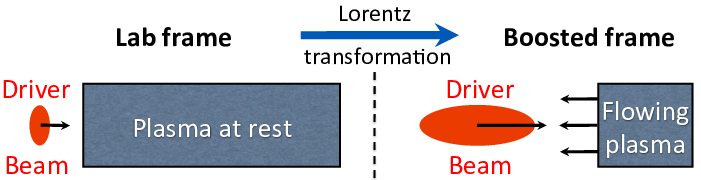
\includegraphics[scale=0.6]{figures/Boosted_frame.png}
%\par\end{centering}
\caption{\label{fig:PIC} A first principle simulation of a short driver beam (laser or charged particles) propagating through a plasma that is orders of magnitude longer necessitates a very large number of time steps. Recasting the simulation in a frame of reference that is moving close to the speed of light in the direction of the driver beam leads to simulating a driver beam that appears longer propagating through a plasma that appears shorter than in the laboratory. Thus, this relativistic transformation of space and time reduces the disparity of scales, and thereby the number of time steps to complete the simulation, by orders of magnitude.}
\end{figure}

Even using a moving window, however, a full PIC simulation of a plasma accelerator can be extraordinarily demanding computationally, as many time steps are needed to resolve the crossing of the short driver beam with the plasma column. As it turns out, choosing an optimal frame of reference that travels close to the speed of light in the direction of the laser or particle beam (as opposed to the usual choice of the laboratory frame) enables speedups by orders of magnitude \cite{Vayprl07,Vaypop2011}. This is a result of the properties of Lorentz contraction and dilation of space and time. In the frame of the laboratory, a very short driver (laser or particle) beam propagates through a much longer plasma column, necessitating millions to tens of millions of time steps for parameters in the range of the BELLA or FACET-II experiments. As sketched in Fig. \ref{fig:PIC}, in a frame moving with the driver beam in the plasma at velocity $v=\beta c$ (where $c$ is the speed of light in vacuum), the beam length is now elongated by $\approx(1+\beta)\gamma$ while the plasma contracts by $\gamma$ (where $\gamma=1/\sqrt{1-\beta^2}$ is the relativistic factor associated with the frame velocity). The number of time steps that is needed to simulate a ``longer'' beam through a ``shorter'' plasma is now reduced by up to $\approx(1+\beta) \gamma^2$ (a detailed derivation of the speedup is given below). 

The modeling of a plasma acceleration stage in a boosted frame 
involves the fully electromagnetic modeling of a plasma propagating at near the speed of light, for which Numerical Cerenkov 
\cite{Borisjcp73,Habericnsp73} is a potential issue, as explained in more details below.
In addition, for a frame of reference moving in the direction of the accelerated beam (or equivalently the wake of the laser), 
waves emitted by the plasma in the forward direction expand 
while the ones emitted in the backward direction contract, following the properties of the Lorentz transformation. 
If one had to resolve both forward and backward propagating 
waves emitted from the plasma, there would be no gain in selecting a frame different from the laboratory frame. However, 
the physics of interest for a laser wakefield is the laser driving the wake, the wake, and the accelerated beam. 
Backscatter is weak in the short-pulse regime, and does not 
interact as strongly with the beam as do the forward propagating waves 
which stay in phase for a long period. It is thus often assumed that the backward propagating waves 
can be neglected in the modeling of plasma accelerator stages. The accuracy  of this assumption has been demonstrated by 
comparison between explicit codes which include both forward and backward waves and envelope or quasistatic codes which neglect backward waves 
\cite{Geddesjp08,Geddespac09,Cowanaac08}.

%%%%%%%%%%%%%%%%%%%%%%%%%%%%%%%%%%%
\subsection{Theoretical speedup dependency with the frame boost}
%%%%%%%%%%%%%%%%%%%%%%%%%%%%%%%%%%%
The derivation that is given here reproduces the one given in \cite{Vaypop2011}, where the obtainable speedup is derived as an extension of the formula that was derived earlier\cite{Vayprl07}, taking in addition into account the group velocity of the laser as it traverses the plasma.  

Assuming that the simulation box is a fixed number of plasma periods long, which implies the use (which is standard) of a moving window following 
the wake and accelerated beam, the speedup is given by the ratio of the time taken by the laser pulse and the plasma to cross each other, divided by the shortest time scale of interest, that is the laser period. To first order, the wake velocity $v_w$ is set by the 1D group velocity of the laser driver, which in the linear (low intensity) limit, is given by \cite{Esareyrmp09}:

%
\begin{equation}
v_w/c=\beta_w=\left(1-\frac{\omega_p^2}{\omega^2}\right)^{1/2}
\end{equation}
%
where $\omega_p=\sqrt{(n_e e^2)/(\epsilon_0 m_e)}$ is the plasma frequency, $\omega=2\pi c/\lambda$ is the laser frequency, $n_e$ is the plasma density, $\lambda$ is the laser wavelength in vacuum, $\epsilon_0$ is the permittivity of vacuum, $c$ is the speed of light in vacuum, and $e$ and $m_e$ are respectively the charge and mass of the electron.

In practice, the runs are typically stopped when the last electron beam macro-particle exits the plasma, and a measure of the total time of the simulation is then given by
%
\begin{equation}
T=\frac{L+\eta \lambda_p}{v_w-v_p}
\end{equation}
%
where $\lambda_p\approx 2\pi c/\omega_p$ is the wake wavelength, $L$ is the plasma length, $v_w$ and $v_p=\beta_p c$ are respectively the velocity of the wake and of the plasma relative to the frame of reference, and $\eta$ is an adjustable parameter for taking into account the fraction of the wake which exited the plasma at the end of the simulation.
For a beam injected into the $n^{th}$ bucket, $\eta$ would be set to $n-1/2$. If positrons were considered, they would be injected half a wake period ahead of the location of the electrons injection position for a given period, and one would have $\eta=n-1$. The numerical cost $R_t$ scales as the ratio of the total time to the shortest timescale of interest, which is the inverse of the laser frequency, and is thus given by
%
\begin{equation}
R_t=\frac{T c}{\lambda}=\frac{\left(L+\eta \lambda_p\right)}{\left(\beta_w-\beta_p\right) \lambda}
\end{equation}
%
In the laboratory, $v_p=0$ and the expression simplifies to 
%
\begin{equation}
R_{lab}=\frac{T c}{\lambda}=\frac{\left(L+\eta \lambda_p\right)}{\beta_w \lambda}
\end{equation}
%
In a frame moving at $\beta c$, the quantities become
\begin{eqnarray}
\lambda_p^*&=&\lambda_p/\left[\gamma \left(1-\beta_w \beta\right)\right] \\
L^*&=&L/\gamma \\
\lambda^*&=& \gamma\left(1+\beta\right) \lambda\\
\beta_w^*&=&\left(\beta_w-\beta\right)/\left(1-\beta_w\beta\right) \\
v_p^*&=&-\beta c \\
T^*&=&\frac{L^*+\eta \lambda_p^*}{v_w^*-v_p^*} \\
R_t^*&=&\frac{T^* c}{\lambda^*} = \frac{\left(L^*+\eta \lambda_p^*\right)}{\left(\beta_w^*+\beta\right) \lambda^*}
\end{eqnarray}
where $\gamma=1/\sqrt{1-\beta^2}$.

The expected speedup from performing the simulation in a boosted frame is given by the ratio of $R_{lab}$ and $R_t^*$
%
\begin{equation}
S=\frac{R_{lab}}{R_t^*}=\frac{\left(1+\beta\right)\left(L+\eta \lambda_p\right)}{\left(1-\beta\beta_w\right)L+\eta \lambda_p}
\label{Eq_scaling1d0}
\end{equation}

We note that assuming that $\beta_w\approx1$ (which is a valid approximation for most practical cases of interest) and that $\gamma<<\gamma_w$, this expression is consistent with the expression derived earlier \cite{Vayprl07} for the laser-plasma acceleration case, which states that $R_t^*=\alpha R_t/\left(1+\beta\right)$ with $\alpha=\left(1-\beta+l/L\right)/\left(1+l/L\right)$, where $l$ is the laser length which is generally proportional to $\eta \lambda_p$, and $S=R_t/R_T^*$. However, higher values of $\gamma$ are of interest for maximum speedup, as shown below.

For intense lasers ($a\sim 1$) typically used for acceleration, the energy gain is limited by dephasing \cite{Schroederprl2011}, which occurs over a scale length $L_d \sim \lambda_p^3/2\lambda^2$.  
Acceleration is compromised beyond $L_d$ and in practice, the plasma length is proportional to the dephasing length, i.e. $L= \xi L_d$. In most cases, $\gamma_w^2>>1$, which allows the approximations $\beta_w\approx1-\lambda^2/2\lambda_p^2$, and $L=\xi \lambda_p^3/2\lambda^2\approx \xi \gamma_w^2 \lambda_p/2>>\eta \lambda_p$, so that Eq.(\ref{Eq_scaling1d0}) becomes
%
\begin{equation}
S=\left(1+\beta\right)^2\gamma^2\frac{\xi\gamma_w^2}{\xi\gamma_w^2+\left(1+\beta\right)\gamma^2\left(\xi\beta/2+2\eta\right)}
\label{Eq_scaling1d}
\end{equation}
%
For low values of $\gamma$, i.e. when $\gamma<<\gamma_w$, Eq.(\ref{Eq_scaling1d}) reduces to
%
\begin{equation}
S_{\gamma<<\gamma_w}=\left(1+\beta\right)^2\gamma^2
\label{Eq_scaling1d_simpl2}
\end{equation}
%
Conversely, if $\gamma\rightarrow\infty$, Eq.(\ref{Eq_scaling1d}) becomes
%
\begin{equation}
S_{\gamma\rightarrow\infty}=\frac{4}{1+4\eta/\xi}\gamma_w^2
\label{Eq_scaling_gamma_inf}
\end{equation}
%
Finally, in the frame of the wake, i.e. when $\gamma=\gamma_w$, assuming that $\beta_w\approx1$, Eq.(\ref{Eq_scaling1d}) gives
%
\begin{equation}
S_{\gamma=\gamma_w}\approx\frac{2}{1+2\eta/\xi}\gamma_w^2
\label{Eq_scaling_gamma_wake}
\end{equation}
Since $\eta$ and $\xi$ are of order unity, and the practical regimes of most interest satisfy $\gamma_w^2>>1$, the speedup that is obtained by using the frame of the wake will be near the maximum obtainable value given by Eq.(\ref{Eq_scaling_gamma_inf}).

Note that without the use of a moving window, the relativistic effects that are at play in the time domain would also be at play in the spatial domain \cite{Vayprl07}, and the $\gamma^2$ scaling would transform to $\gamma^4$. Hence, it is important to use a moving window even in simulations in a Lorentz boosted frame. For very high values of the boosted frame, the optimal velocity of the moving window may vanish (i.e. no moving window) or even reverse.

%%%%%%%%%%%%%%%%%%%%%%%%%%%%%%%%%%%
\subsection{Numerical Stability and alternate formulation in a Galilean frame}
%%%%%%%%%%%%%%%%%%%%%%%%%%%%%%%%%%%

The numerical Cherenkov instability (NCI) \cite{Godfreyjcp74}
is the most serious numerical instability affecting multidimensional
PIC simulations of relativistic particle beams and streaming plasmas
\cite{Martinscpc10,VayAAC2010,Vayjcp2011,Spitkovsky:Icnsp2011,GodfreyJCP2013,XuJCP2013}. 
It arises from coupling between possibly numerically distorted electromagnetic modes and spurious
beam modes, the latter due to the mismatch between the Lagrangian
treatment of particles and the Eulerian treatment of fields \cite{Godfreyjcp75}.

In recent papers the electromagnetic dispersion
relations for the numerical Cherenkov instability were derived and solved for both FDTD \cite{GodfreyJCP2013,GodfreyJCP2014_FDTD}
and PSATD \cite{GodfreyJCP2014_PSATD,GodfreyIEEE2014} algorithms. 

Several solutions have been proposed to mitigate the NCI \cite{GodfreyJCP2014,GodfreyIEEE2014,GodfreyJCP2014_PSATD,GodfreyCPC2015,YuCPC2015,YuCPC2015-Circ}. Although
these solutions efficiently reduce the numerical instability,
they typically introduce either strong smoothing of the currents and
fields, or arbitrary numerical corrections, which are
tuned specifically against the NCI and go beyond the
natural discretization of the underlying physical equation. Therefore,
it is sometimes unclear to what extent these added corrections could impact the
physics at stake for a given resolution.

For instance, NCI-specific corrections include periodically smoothing 
the electromagnetic field components \cite{Martinscpc10}, 
using a special time step \cite{VayAAC2010,Vayjcp2011} or
applying a wide-band smoothing of the current components \cite{
  VayAAC2010,Vayjcp2011,VayPOPL2011}. Another set of mitigation methods
involve scaling the deposited
currents by a carefully-designed wavenumber-dependent factor
\cite{GodfreyJCP2014_FDTD,GodfreyIEEE2014} or slightly modifying the
ratio of electric and magnetic fields ($E/B$) before gathering their
value onto the macroparticles 
\cite{GodfreyJCP2014_PSATD,GodfreyCPC2015}. 
Yet another set of NCI-specific corrections
\cite{YuCPC2015,YuCPC2015-Circ} consists 
in combining a small timestep $\Delta t$, a sharp low-pass spatial filter,
and a spectral or high-order scheme that is tuned so as to
create a small, artificial ``bump'' in the dispersion relation
\cite{YuCPC2015}. While most mitigation methods have only been applied
to Cartesian geometry, this last
set of methods (\cite{YuCPC2015,YuCPC2015-Circ}) 
has the remarkable property that it can be applied
\cite{YuCPC2015-Circ} to both Cartesian geometry and
quasi-cylindrical geometry (i.e. cylindrical geometry with
azimuthal Fourier decomposition \cite{LifschitzJCP2009,DavidsonJCP2015,Lehe2016}). However,
the use of a small timestep proportionally slows down the progress of
the simulation, and the artificial ``bump'' is again an arbitrary correction
that departs from the underlying physics.

A new scheme was recently proposed, in \cite{KirchenARXIV2016,LeheARXIV2016}, which 
completely eliminates the NCI for a plasma drifting at a uniform relativistic velocity 
-- with no arbitrary correction -- by simply integrating
the PIC equations in \emph{Galilean coordinates} (also known as
\emph{comoving coordinates}). More precisely, in the new 
method, the Maxwell equations \emph{in Galilean coordinates} are integrated
analytically, using only natural hypotheses, within the PSATD
framework (Pseudo-Spectral-Analytical-Time-Domain \cite{Habericnsp73,VayJCP2013}). 

The idea of the proposed scheme is to perform a Galilean change of
coordinates, and to carry out the simulation in the new coordinates:
\begin{equation} 
\label{eq:change-var}
\vec{x}' = \vec{x} - \vgal t 
\end{equation}
where $\vec{x} = x\,\vec{u}_x + y\,\vec{u}_y + z\,\vec{u}_z$ and
$\vec{x}' = x'\,\vec{u}_x + y'\,\vec{u}_y + z'\,\vec{u}_z$ are the
position vectors in the standard and Galilean coordinates
respectively.

When choosing $\vgal= \vec{v}_0$, where
$\vec{v}_0$ is the speed of the bulk of the relativistic
plasma, the plasma does not move with respect to the grid in the Galilean 
coordinates $\vec{x}'$ -- or, equivalently, in the standard
coordinates $\vec{x}$, the grid moves along with the plasma. The heuristic intuition behind this scheme
is that these coordinates should prevent the discrepancy between the Lagrangian and
Eulerian point of view, which gives rise to the NCI \cite{Godfreyjcp75}.

An important remark is that the Galilean change of
coordinates (\ref{eq:change-var}) is a simple translation. Thus, when used in
the context of Lorentz-boosted simulations, it does
of course preserve the relativistic dilatation of space and time which gives rise to the
characteristic computational speedup of the boosted-frame technique.

Another important remark is that the Galilean scheme is \emph{not}
equivalent to a moving window (and in fact the Galilean scheme can be
independently \emph{combined} with a moving window). Whereas in a
moving window, gridpoints are added and removed so as to effectively
translate the boundaries, in the Galilean scheme the gridpoints
\emph{themselves} are not only translated but in this case, the physical equations
are modified accordingly. Most importantly, the assumed time evolution of
the current $\vec{J}$ within one timestep is different in a standard PSATD scheme with moving
window and in a Galilean PSATD scheme \cite{LeheARXIV2016}.

In the Galilean coordinates $\vec{x}'$, the equations of particle
motion and the Maxwell equations take the form 
\begin{subequations}
\begin{align}
\frac{d\vec{x}'}{dt} &= \frac{\vec{p}}{\gamma m} - \vgal \label{eq:motion1} \\ 
\frac{d\vec{p}}{dt} &= q \left( \vec{E} +
\frac{\vec{p}}{\gamma m} \times \vec{B} \right) \label{eq:motion2}\\
\left( \Dt{\;} - \vgal\cdot\nab\right)\vec{B} &= -\nab\times\vec{E} \label{eq:maxwell1}\\
\frac{1}{c^2}\left( \Dt{\;} - \vgal\cdot\nab\right)\vec{E} &= \nab\times\vec{B} - \mu_0\vec{J} \label{eq:maxwell2}
\end{align}
\end{subequations}
where $\nab$ denotes a spatial derivative with respect to the
Galilean coordinates $\vec{x}'$. 

Integrating these equations from $t=n\Delta
t$ to $t=(n+1)\Delta t$ results in the following update equations (see
\cite{LeheARXIV2016} for the details of the derivation):
%
\begin{subequations}
\begin{align}
%
\fb^{n+1} &= \theta^2 C \fb^n
 -\frac{\theta^2 S}{ck}i\vec{k}\times \fe^n \nonumber \\
& + \;\frac{\theta \chi_1}{\epsilon_0c^2k^2}\;i\vec{k} \times
                     \fj^{n+1/2} \label{eq:disc-maxwell1}\\
%
\fe^{n+1} &=  \theta^2 C  \fe^n
 +\frac{\theta^2 S}{k} \,c i\vec{k}\times \fb^n \nonumber \\
& +\frac{i\nu \theta \chi_1 - \theta^2S}{\epsilon_0 ck} \; \fj^{n+1/2}\nonumber \\
& - \frac{1}{\epsilon_0k^2}\left(\; \chi_2\;\mc{\rho}^{n+1} -
  \theta^2\chi_3\;\mc{\rho}^{n} \;\right) i\vec{k} \label{eq:disc-maxwell2}
%
\end{align}
\end{subequations}
%
where we used the short-hand notations $\fe^n \equiv
%
\fe(\vec{k}, n\Delta t)$, $\fb^n \equiv
\fb(\vec{k}, n\Delta t)$ as well as:
\begin{subequations}
\begin{align}
&C = \cos(ck\Delta t) \quad S = \sin(ck\Delta t) \quad k
= |\vec{k}| \label{eq:def-C-S}\\&
\nu = \frac{\vec{k}\cdot\vgal}{ck} \quad \theta =
  e^{i\vec{k}\cdot\vgal\Delta t/2} \quad \theta^* =
  e^{-i\vec{k}\cdot\vgal\Delta t/2} \label{eq:def-nu-theta}\\&
\chi_1 =  \frac{1}{1 -\nu^2} \left( \theta^* -  C \theta + i
  \nu \theta S \right) \label{eq:def-chi1}\\&
\chi_2 = \frac{\chi_1 - \theta(1-C)}{\theta^*-\theta} \quad
\chi_3 = \frac{\chi_1-\theta^*(1-C)}{\theta^*-\theta} \label{eq:def-chi23}
\end{align}
\end{subequations}
Note that, in the limit $\vgal=\vec{0}$,
(\ref{eq:disc-maxwell1}) and (\ref{eq:disc-maxwell2}) reduce to the standard PSATD
equations \cite{Habericnsp73}, as expected. 
As shown in \cite{KirchenARXIV2016,LeheARXIV2016}, 
the elimination of the NCI with the new Galilean integration is verified empirically via PIC simulations of uniform drifting plasmas and laser-driven plasma acceleration stages, and confirmed by a theoretical analysis of the instability.

%%%%%%%%%%%%%%%%%%%%%%%%%%%%%%%%%%%
\section{Axi-symmetry and azimuthal Fourier decomposition}
%%%%%%%%%%%%%%%%%%%%%%%%%%%%%%%%%%%

Although full PIC codes are powerful tools, which capture a wide range
of physical phenomena, they also require large computational ressources. 
This is partly due to the use of a 3D Cartesian grid, which
leads to a very large number of grid cells. (Typical 3D simulations of
laser-wakefield acceleration require $\sim 10^6$--$ 10^8$ grid
cells.) For this reason, these algorithms need to be highly parallelized, and
high-resolution simulations can only be run on costly large-scale
computer facilities. However, when the driver is
cylindrically-symmetric, it is possible to take advantage of the
symmetry of the problem to reduce the computational cost of the algorithm \cite{godfrey1985iprop,LifschitzJCP2009,DavidsonJCP2015,Lehe2016}.

\subsection{Azimuthal decomposition}
Let us consider the fields $\vec{E}$, $\vec{B}$, $\vec{J}$ and $\rho$
 in cylindral coordinates $(r,\theta,z)$, expressed as a Fourier series in $\theta$:
%
\begin{equation}
F(r,\theta,z) = \mathrm{Re}\left[ \sum_{\ell=0}^\infty
  \tilde{F}_{\ell}(r,z) e^{-i\ell\theta} \right] 
\label{eq:chap2:azimuthal}
\end{equation}
%
\begin{equation}
\mathrm{with} \qquad \tilde{F}_{\ell} = C_\ell \int_0^{2\pi} d\theta
\,F(r,\theta,z)e^{i\ell\theta} \qquad 
\label{eq:chap2:Fourier-coeffs}
\end{equation}
\begin{equation}
\mathrm{and} \;
\left \{ \begin{array}{l l}
C_{0} = 1/2\pi &\\
C_\ell = 1/\pi &\mathrm{for}\,\ell > 0
\end{array} \right.
\end{equation}
%
where $F$ represents any of the quantities $E_r$,
$E_\theta$, $E_z$, $B_r$, $B_\theta$, $B_z$, $J_r$, $J_\theta$, $J_z$
are $\rho$, and where the
$\tilde{F}_\ell$ are the associated Fourier components ($\ell$ is the
index of the corresponding azimuthal mode). In the general case, this
azimuthal decomposition does not simplify the problem, since an
infinity of modes have to be considered in (\ref{eq:chap2:azimuthal}). However, in the case of a
cylindrically-symmetric laser pulse, only the very first modes have
non-zero components. For instance, the wakefield is represented
exclusively by the mode $\ell = 0$. (This is because the quantities $E_r$,
$E_\theta$, $E_z$, $B_r$, $B_\theta$, $B_z$, $J_r$, $J_\theta$, $J_z$
and $\rho$ associated with the
wakefield are independent of $\theta$.) On the other hand, the field
of the laser pulse \emph{does}
depend on $\theta$, in cylindrical coordinates. For example, for a
cylindrically-symmetric pulse propagating along $z$ and polarized along $\vec{e}_\alpha = \cos(\alpha)\vec{e}_x + \sin(\alpha)\vec{e}_y$:
%
\begin{align}
\vec{E} &= E_0(r,z)\vec{e}_\alpha \\
& = E_0(r,z) [\; \cos(\alpha)(\cos(\theta)\vec{e}_r - \sin(\theta)\vec{e}_\theta) \; \nonumber \\ 
& + \; \sin(\alpha)(\sin(\theta)\vec{e}_r + \cos(\theta)\vec{e}_\theta) \; ]\\
& = \mathrm{Re}[ \; E_0(r,z) e^{i\alpha} e^{-i\theta} \; ]\vec{e}_r \; \nonumber \\
& + \; \mathrm{Re}[ \; -i E_0(r,z) e^{i\alpha} e^{-i\theta} \; ]\vec{e}_\theta.
\end{align}
%
Here the amplitude $E_0$ does not depend on $\theta$ because the pulse was assumed
to be cylindrically symmetric. In this case, the above relation shows
that the fields $E_r$ and $E_\theta$ of the laser are represented
exclusively by the mode $\ell = 1$. A similar calculation shows that
the same holds for $B_r$ and $B_\theta$. On the whole, only the modes
$\ell = 0$ and $\ell = 1$ are a priori necessary to model
laser-wakefield acceleration. 
Under those conditions, the infinite sum in
(\ref{eq:chap2:azimuthal}) is truncated at a chosen $\ell_{max}$. In
principle, $\ell_{max} = 1$ is sufficient for laser-wakefield
acceleration. However, $\ell_{max}$ is kept as a free parameter in the algorithm, in order to verify that
higher modes are negligible, as well as to allow for less-symmetric configurations. 
Because codes based on this algorithm are able to take into account the modes with $\ell > 0$, they are said to be
``quasi-cylindrical'' (or ``quasi-3D'' by some authors \cite{DavidsonJCP2015}), in contrast to cylindrical codes, which
assume that all fields are independent of $\theta$, and thus only
consider the mode $\ell = 0$.

\subsection{Discretized Maxwell equations} When the Fourier expressions
of the fields are injected into the Maxwell equations (written in
cylindrical coordinates), the different azimuthal modes
decouple. In this case, the Maxwell-Amp\`ere and Maxwell-Faraday equations
-- which are needed to update the fields in the PIC cycle -- can be written separately
for each azimuthal mode $\ell$:
\begin{subequations}
\begin{align}
\frac{\partial \tilde{B}_{r,\ell} }{\partial t} &=
\frac{i\ell}{r}\tilde{E}_{z,\ell} + \frac{\partial
  \tilde{E}_{\theta,\ell}}{\partial z} \\[3mm]
\frac{\partial \tilde{B}_{\theta,\ell} }{\partial t} &=
 - \frac{\partial \tilde{E}_{r,\ell}}{\partial z} + \frac{\partial
  \tilde{E}_{z,\ell}}{\partial r} \\[3mm]
\frac{\partial \tilde{B}_{z,\ell} }{\partial t} &=
- \frac{1}{r} \frac{\partial (r\tilde{E}_{\theta,\ell})}{\partial r} - \frac{i\ell}{r}\tilde{E}_{r,\ell} \\[3mm]
\frac{1}{c^2} \frac{\partial \tilde{E}_{r,\ell} }{\partial t} &=
-\frac{i\ell}{r}\tilde{B}_{z,\ell} - \frac{\partial
  \tilde{B}_{\theta,\ell}}{\partial z} - \mu_0 \tilde{J}_{r,\ell} \\[3mm]
\frac{1}{c^2}\frac{\partial \tilde{E}_{\theta,\ell} }{\partial t} &=
 \frac{\partial \tilde{B}_{r,\ell}}{\partial z} - \frac{\partial
  \tilde{B}_{z,\ell}}{\partial r} - \mu_0 \tilde{J}_{\theta,\ell} \\[3mm]
\frac{1}{c^2}\frac{\partial \tilde{E}_{z,\ell} }{\partial t} &=
 \frac{1}{r} \frac{\partial (r\tilde{B}_{\theta,\ell})}{\partial r} +
 \frac{i\ell}{r}\tilde{B}_{r,\ell} - \mu_0 \tilde{J}_{z,\ell}
\end{align}
\end{subequations}
%\begin{figure}
%\input{./Chap2/Circ_lattice.tex}
%\caption{Representation of the lattice in \CCirc. The
%  table shows at which
%  position each component of the fields is defined ($j$,$k$ and
%  $n$ are integers ; $\Delta r$ and $\Delta z$ are the
%  spatial steps of the grid). The above sketch represents one grid
%  cell, and the positions of the fields within it.}
%\label{fig:chap2:Circ_lattice}
%\end{figure}
In order to discretize these equations, each azimuthal mode is
represented on a two-dimensional grid, 
%(The two dimensions correspond
%to $r$ and $z$.) \Cref{fig:chap2:Circ_lattice} summarizes the
%positions of the different fields within one grid cell, as well as the
%corresponding notations for these fields. Using these notations, 
on which the discretized
Maxwell-Amp\`ere and Maxwell-Faraday equations are given by
%\begin{strip}
%\begin{align*}
%
%\frac{ \tBr{n+\hf}{j,\ell,k+\hf}- \tBr{n-\hf}{j,\ell,k+\hf} 
%}{\Delta t} =& \frac{i\,\ell}{j\Delta r}\tEz{n}{j,\ell,k+\hf} + (D_z \tilde{E}_{\theta}^n)_{j,\ell,k+\hf} \\
%
%\frac{ \tBt{n+\hf}{j+\hf,\ell,k+\hf}- \tBt{n-\hf}{j+\hf,\ell,k+\hf} }{\Delta t} =& -(D_z \tilde{E}_r^n)_{j+\hf,\ell,k+\hf} + (D_r \tilde{E}_z^{n})_{j+\hf,\ell,k+\hf} \\
%
%\frac{ \tBz{n+\hf}{j+\hf,\ell,k}- \tBz{n-\hf}{j+\hf,\ell,k} }{\Delta t} =&  
% -\frac{(j+1)\tEt{n}{j+1,\ell,k} - j\tEt{n}{j,\ell,k}}{(j+\hf)\Delta r} -
%\frac{i\,\ell}{(j+\hf) \Delta r}\tEr{n}{j+\hf,\ell,k} \\
%
%\frac{ \tEr{n+1}{j+\hf,\ell,k}- \tEr{n}{j+\hf,\ell,k}}{c^2 \Delta t} 
%=& -\frac{i\,\ell}{(j+\hf)\Delta r}\tBz{n+\hf}{j+\hf,\ell,k} - (D_z \tilde{B}_{\theta}^{n+\hf})_{j+\hf,\ell,k} - \mu_0\tJr{n+\hf}{j+\hf,\ell,k} \\
%
%\frac{ \tEt{n+1}{j,\ell,k}- \tEt{n}{j,\ell,k}}{c^2 \Delta t} 
%=& (D_z \tilde{B}_r^{n+\hf})_{j,\ell,k} - (D_r \tilde{B}_z^{n+\hf})_{j,\ell,k} - \mu_0\tJt{n+\hf}{j,\ell,k} \\
%
%\frac{ \tEz{n+1}{j,\ell,k+\hf}- \tEz{n}{j,\ell,k+\hf}}{c^2 \Delta t} 
%=&   \frac{\left(j+\hf\right)\tBt{n+\hf}{j+\hf,\ell,k+\hf}  - \left(j-\hf\right)\tBt{n+\hf}{j-\hf,\ell,k+\hf}}{j\Delta r} \\
%& \qquad  \qquad + \frac{i\,\ell}{j\Delta r}\tBr{n+\hf}{j,\ell,k+\hf} - \mu_0\tJz{n+\hf}{j,\ell,k+\hf}
%\end{align*}
%\end{strip}

\begin{subequations}
\begin{align}
%
D_{t}\tilde{B}_r|_{j,\ell,k+\hf}^{n} \nonumber
=& \frac{i\,\ell}{j\Delta r}\tEz{n}{j,\ell,k+\hf} \\ 
& + D_z \tilde{E}_{\theta}|^n_{j,\ell,k+\hf} \\
%
D_{t}\tilde{B}_\theta|_{j+\hf,\ell,k+\hf}^{n} \nonumber
=& -D_z \tilde{E}_r|^n_{j+\hf,\ell,k+\hf} \\
& + D_r \tilde{E}_z|^{n}_{j+\hf,\ell,k+\hf} \\
%
D_{t}\tilde{B}_z|_{j+\hf,\ell,k}^{n} =& \nonumber
 -\frac{(j+1)\tEt{n}{j+1,\ell,k} }{(j+\hf)\Delta r} \\ \nonumber
 & +\frac{ j\tEt{n}{j,\ell,k}}{(j+\hf)\Delta r} \\
 & - \frac{i\,\ell}{(j+\hf) \Delta r}\tEr{n}{j+\hf,\ell,k} 
\end{align}
\end{subequations}
for the magnetic field components, and 
\begin{subequations}
\begin{align}
%
\frac{1}{c^2}D_{t}\tilde{E}_r|_{j+\hf,\ell,k}^{n+\hf} \nonumber
=& -\frac{i\,\ell}{(j+\hf)\Delta r}\tBz{n+\hf}{j+\hf,\ell,k} \\
& - D_z \tilde{B}_{\theta}|^{n+\hf}_{j+\hf,\ell,k} \nonumber\\
& - \mu_0\tJr{n+\hf}{j+\hf,\ell,k} \\
%
\frac{1}{c^2}D_{t}\tilde{E}_\theta|_{j,\ell,k}^{n+\hf} \nonumber
=& D_z \tilde{B}_r|^{n+\hf}_{j,\ell,k} - D_r \tilde{B}_z|^{n+\hf}_{j,\ell,k} \\
& - \mu_0\tJt{n+\hf}{j,\ell,k} \\
%
\frac{1}{c^2}D_{t}\tilde{E}_z|_{j,\ell,k+\hf}^{n+\hf} \nonumber
=&   \frac{\left(j+\hf\right)\tBt{n+\hf}{j+\hf,\ell,k+\hf} }{j\Delta r} \\
=&   -\frac{\left(j-\hf\right)\tBt{n+\hf}{j-\hf,\ell,k+\hf}}{j\Delta r} \nonumber\\
& + \frac{i\,\ell}{j\Delta r}\tBr{n+\hf}{j,\ell,k+\hf} \nonumber\\
& - \mu_0\tJz{n+\hf}{j,\ell,k+\hf}
\end{align}
\end{subequations}
for the electric field components.

The numerical operator $D_r$ and $D_z$ are defined by
\begin{align*} 
(D_r F)_{j',\ell,k'} = \frac{F_{j'+\hf,\ell,k'}-F_{j'-\hf,\ell,k'} }{\Delta r} \\ 
(D_z F)_{j',\ell,k'} = \frac{F_{j',\ell,k'+\hf}-F_{j',\ell,k'-\hf} }{\Delta z} \\ 
\end{align*}
where $j'$ and $k'$ can be integers or half-integers. Notice 
that these discretized Maxwell equations are not valid on-axis (i.e. for $j=0$), due to
singularities in some of the terms. Therefore, on the axis, these equations are replaced by specific boundary conditions, which are based on the symmetry properties of the fields (see \cite{LifschitzJCP2009} for details).

Compared to a 3D Cartesian calculation with $n_x\times n_y \times n_z$  
grid cells, a quasi-cylindrical calculation with two modes ($l=0$ and $l=1$) 
will require only $3 \,n_r \times n_z$ grid cells. Assuming $n_x=n_y=n_r=100$ 
as a typical transverse resolution, a quasi-cylindrical calculation is typically 
over an order of magnitude less computationally demanding than its 3D Cartesian 
equivalent.

%%%%%%%%%%%%%%%%%%%%%%%%%%%%%%%%%%%
\section{Filtering}
%%%%%%%%%%%%%%%%%%%%%%%%%%%%%%%%%%%

It is common practice to apply digital filtering to the charge or
current density in Particle-In-Cell simulations as a complement or
an alternative to using higher order splines \cite{Birdsalllangdon}.
A commonly used filter in PIC simulations is the three points filter
$\phi_{j}^{f}=\alpha\phi_{j}+\left(1-\alpha\right)\left(\phi_{j-1}+\phi_{j+1}\right)/2$
where $\phi^{f}$ is the filtered quantity. This filter is called
a bilinear filter when $\alpha=0.5$. Assuming $\phi=e^{jkx}$ and
$\phi^{f}=g\left(\alpha,k\right)e^{jkx}$, the filter gain $g$ is
given as a function of the filtering coefficient $\alpha$ and
the wavenumber $k$ by $g\left(\alpha,k\right)=\alpha+\left(1-\alpha\right)\cos\left(k\Delta x\right)\approx1-\left(1-\alpha\right)\frac{\left(k\Delta x\right)^{2}}{2}+O\left(k^{4}\right)$.
The total attenuation $G$ for $n$ successive applications of filters
of coefficients $\alpha_{1}$...$\alpha_{n}$ is given by $G=\prod_{i=1}^{n}g\left(\alpha_{i},k\right)\approx1-\left(n-\sum_{i=1}^{n}\alpha_{i}\right)\frac{\left(k\Delta x\right)^{2}}{2}+O\left(k^{4}\right)$.
A sharper cutoff in $k$ space is provided by using $\alpha_{n}=n-\sum_{i=1}^{n-1}\alpha_{i}$,
so that $G\approx1+O\left(k^{4}\right)$. Such step is called a ``compensation''
step \cite{Birdsalllangdon}. For the bilinear filter ($\alpha=1/2$),
the compensation factor is $\alpha_{c}=2-1/2=3/2$. For a succession
of $n$ applications of the bilinear factor, it is $\alpha_{c}=n/2+1$. 

It is sometimes necessary to filter on a relatively wide band of wavelength,
necessitating the application of a large number of passes of the bilinear
filter or on the use of filters acting on many points. The former
can become very intensive computationally while the latter is problematic
for parallel computations using domain decomposition, as the footprint
of the filter may eventually surpass the size of subdomains. A workaround
is to use a combination of filters of limited footprint. A solution
based on the combination of three point filters with various strides
was proposed in \cite{Vayjcp2011} and operates as follows. 

The bilinear filter provides complete suppression of the signal at
the grid Nyquist wavelength (twice the grid cell size). Suppression
of the signal at integer multiples of the Nyquist wavelength can be
obtained by using a stride $s$ in the filter $\phi_{j}^{f}=\alpha\phi_{j}+\left(1-\alpha\right)\left(\phi_{j-s}+\phi_{j+s}\right)/2$
for which the gain is given by $g\left(\alpha,k\right)=\alpha+\left(1-\alpha\right)\cos\left(sk\Delta x\right)\approx1-\left(1-\alpha\right)\frac{\left(sk\Delta x\right)^{2}}{2}+O\left(k^{4}\right)$.
For a given stride, the gain is given by the gain of the bilinear
filter shifted in k space, with the pole $g=0$ shifted from the wavelength
$\lambda=2/\Delta x$ to $\lambda=2s/\Delta x$, with additional poles,
as given by $sk\Delta x=\arccos\left(\frac{\alpha}{\alpha-1}\right)\pmod{2\pi}$.
The resulting filter is pass band between the poles, but since the
poles are spread at different integer values in k space, a wide band
low pass filter can be constructed by combining filters using different
strides. As shown in \cite{Vayjcp2011}, the successive application
of 4-passes + compensation of filters with strides 1, 2 and 4 has
a nearly equivalent fall-off in gain as 80 passes + compensation of
a bilinear filter. Yet, the strided filter solution needs only 15
passes of a three-point filter, compared to 81 passes for an equivalent
n-pass bilinear filter, yielding a gain of 5.4 in number of operations
in favor of the combination of filters with stride. The width of the
filter with stride 4 extends only on 9 points, compared to 81 points
for a single pass equivalent filter, hence giving a gain of 9 in compactness
for the stride filters combination in comparison to the single-pass
filter with large stencil, resulting in more favorable scaling with the number 
of computational cores for parallel calculations.

%%%%%%%%%%%%%%%%%%%%%%%%%%%%%%%%%%
%\section{Porting onto new architectures, parallelization, vectorization, mesh refinement}
%%%%%%%%%%%%%%%%%%%%%%%%%%%%%%%%%%

%%%%%%%%%%%%%%%%%%%%%%%%%%%%%%%%%%%
\section{Inputs and outputs}
%%%%%%%%%%%%%%%%%%%%%%%%%%%%%%%%%%%

Initialization of the plasma columns and drivers (laser or particle beam) is performed via the specification of multidimensional functions that describe the initial state with, if needed, a time dependence, or from reconstruction of distributions based on experimental data. Care is needed when initializing quantities in parallel to avoid double counting and ensure smoothness of the distributions at the interface of computational domains. When the sum of the initial distributions of charged particles is not charge neutral, initial fields are computed using generally a static approximation with Poisson solves accompanied by proper relativistic scalings \cite{Vaypop2008, CowanPRSTAB13}. 

Outputs include dumps of particle and field quantities at regular intervals, histories of particle distributions moments, spectra, etc, and plots of the various quantities. In parallel simulations, the diagnostic subroutines need to handle additional complexity from the domain decomposition, as well as large amount of data that may necessitate data reduction in some form before saving to disk. 

Simulations in a Lorentz boosted frame require additional considerations, as described below.

\subsection{Inputs and outputs in a boosted frame simulation}
\begin{figure}
%   \centering
   \includegraphics[width=120mm]{figures/Input.png}
   \includegraphics[width=120mm]{figures/Output.png}
   \caption{(color online) (top) Snapshot of a particle beam showing ``frozen" (grey spheres) and ``active" (colored spheres) macroparticles traversing the injection plane (red rectangle). (bottom) Snapshot of the beam macroparticles (colored spheres) passing through the background of electrons (dark brown streamlines) and the diagnostic stations (red rectangles). The electrons, the injection plane and the diagnostic stations are fixed in the laboratory plane, and are thus counter-propagating to the beam in a boosted frame. }
   \label{Fig_inputoutput}
\end{figure}

The input and output data are often known from, or compared to, experimental data. Thus, calculating in 
a frame other than the laboratory entails transformations of the data between the calculation frame and the laboratory 
frame. This section describes the procedures that have been implemented in the Particle-In-Cell framework Warp \cite{Warp} to handle the input and output of data between the frame of calculation and the laboratory frame \cite{Vaypop2011}. Simultaneity of events between two frames is valid only for a plane that is perpendicular to the relative motion of the frame. As a result, the input/output processes involve the input of data (particles or fields) through a plane, as well as output through a series of planes, all of which are perpendicular to the direction of the relative velocity between the frame of calculation and the other frame of choice. 

\subsubsection{Input in a boosted frame simulation}
\paragraph{Particles - }
Particles are launched through a plane using a technique that is generic and applies to Lorentz boosted frame simulations in general, including plasma acceleration, and is illustrated using the case of a positively charged particle beam propagating through a background of cold electrons in an assumed continuous transverse focusing system, leading to a well-known growing transverse ``electron cloud'' instability  \cite{Vayprl07}. In the laboratory frame, the electron background is initially at rest and a moving window is used to follow the beam progression. Traditionally, the beam macroparticles are initialized all at once in the window, while background electron macroparticles are created continuously in front of the beam on a plane that is perpendicular to the beam velocity. In a frame moving at some fraction of the beam velocity in the laboratory frame, the beam initial conditions at a given time in the calculation frame are generally unknown and one must initialize the beam differently. However, it can be taken advantage of the fact that the beam initial conditions are often known for a given plane in the laboratory, either directly, or via simple calculation or projection from the conditions at a given time in the labortory frame. Given the position and velocity $\{x,y,z,v_x,v_y,v_z\}$ for each beam macroparticle at time $t=0$ for a beam moving at the average velocity $v_b=\beta_b c$ (where $c$ is the speed of light) in the laboratory, and using the standard synchronization ($z=z'=0$ at $t=t'=0$) between the laboratory and the calculation frames, the procedure for transforming the beam quantities for injection in a boosted frame moving at velocity $\beta c$ in the laboratory is as follows (the superscript $'$ relates to quantities known in the boosted frame while the superscript $^*$ relates to quantities that are know at a given longitudinal position $z^*$ but different times of arrival):

\begin{enumerate}
\item project positions at $z^*=0$ assuming ballistic propagation
\begin{eqnarray} 
    t^* &=& \left(z-\bar{z}\right)/v_z \label{Eq:t*}\\
    x^* &=& x-v_x t^* \label{Eq:x*}\\
    y^* &=& y-v_y t^* \label{Eq:y*}\\
    z^* &=& 0 \label{Eq:z*}
\end{eqnarray}
the velocity components being left unchanged, 
\item apply Lorentz transformation from laboratory frame to boosted frame
\begin{eqnarray} 
    t'^* &=& -\gamma t^* \label{Eq:tp*}\\
    x'^* &=& x^* \label{Eq:xp*}\\
    y'^* &=& y^* \label{Eq:yp*}\\
    z'^* &=& \gamma\beta c t^* \label{Eq:zp*}\\
    v'^*_x&=&\frac{v_x^*}{\gamma\left(1-\beta \beta_b\right)} \label{Eq:vxp*}\\
    v'^*_y&=&\frac{v_y^*}{\gamma\left(1-\beta \beta_b\right)} \label{Eq:vyp*}\\
    v'^*_z&=&\frac{v_z^*-\beta c}{1-\beta \beta_b} \label{Eq:vzp*}
\end{eqnarray}
where $\gamma=1/\sqrt{1-\beta^2}$. With the knowledge of the time at which each beam macroparticle crosses the plane into consideration, one can inject each beam macroparticle in the simulation at the appropriate location and time. 

\item synchronize macroparticles in boosted frame, obtaining their positions at a fixed $t'=0$ (before any particle is injected)
\begin{eqnarray} 
    z' &=& z'^*-\bar{v}'^*_z t'^* \label{Eq:zp}
\end{eqnarray}
    This additional step is needed for setting the electrostatic or electromagnetic fields at the plane of injection. In a Particle-In-Cell code, the three-dimensional fields are calculated by solving the Maxwell equations (or static approximation like Poisson, Darwin or other \cite{Vaypop2008}) on a grid on which the source term is obtained from the macroparticles distribution. This requires generation of a three-dimensional representation of the beam distribution of macroparticles at a given time before they cross the injection plane at $z'^*$. This is accomplished by expanding the beam distribution longitudinally such that all macroparticles (so far known at different times of arrival at the injection plane) are synchronized to the same time in the boosted frame. To keep the beam shape constant, the particles are ``frozen'' until they cross that plane: the three velocity components and the two position components perpendicular to the boosted frame velocity are kept constant, while the remaining position component is advanced at the average beam velocity. As particles cross the plane of injection, they become regular ``active'' particles with full 6-D dynamics.

\end{enumerate}

Figure \ref{Fig_inputoutput} (top) shows a snapshot of a beam that has passed partly through the injection plane. As the frozen beam macroparticles pass through the injection plane (which moves opposite to the beam in the boosted frame), they are converted to ``active" macroparticles. The charge or current density is accumulated from the active and the frozen particles, thus ensuring that the fields at the plane of injection are consistent. 

\paragraph{Laser - }

Similarly to the particle beam, the laser is injected through a plane perpendicular to the axis of propagation of the laser (by default $z$). 
The electric field $E_\perp$ that is to be emitted is given by the formula
\begin{equation}
E_\perp\left(x,y,t\right)=E_0 f\left(x,y,t\right) \sin\left[\omega t+\phi\left(x,y,\omega\right)\right] 
\end{equation}
where $E_0$ is the amplitude of the laser electric field, $f\left(x,y,t\right)$ is the laser envelope, $\omega$ is the laser frequency, $\phi\left(x,y,\omega\right)$ is a phase function to account for focusing, defocusing or injection at an angle, and $t$ is time. By default, the laser envelope is a three-dimensional gaussian of the form 
\begin{equation}
 f\left(x,y,t\right)=e^{-\left(x^2/2 \sigma_x^2+y^2/2 \sigma_y^2+c^2t^2/2 \sigma_z^2\right)}
 \end{equation}
 where $\sigma_x$, $\sigma_y$ and $\sigma_z$ are the dimensions of the laser pulse; or it can be defined arbitrarily by the user at runtime.
If $\phi\left(x,y,\omega\right)=0$, the laser is injected at a waist and parallel to the axis $z$. 

If, for convenience, the injection plane is moving at constant velocity $\beta_s c$, the formula is modified to take the Doppler effect on frequency and amplitude into account and becomes
\begin{eqnarray}
E_\perp\left(x,y,t\right)&=&\left(1-\beta_s\right)E_0 f\left(x,y,t\right)\nonumber \\
&\times& \sin\left[\left(1-\beta_s\right)\omega t+\phi\left(x,y,\omega\right)\right].
\end{eqnarray}

The injection of a laser of frequency $\omega$ is considered for a simulation using a boosted frame moving at $\beta c$ with respect to the laboratory. Assuming that the laser is injected at a plane that is fixed in the laboratory, and thus moving at $\beta_s=-\beta$ in the boosted frame, the injection in the boosted frame is given by
\begin{eqnarray}
E_\perp\left(x',y',t'\right)&=&\left(1-\beta_s\right)E'_0 f\left(x',y',t'\right)\nonumber \\ 
&\times&\sin\left[\left(1-\beta_s\right)\omega' t'+\phi\left(x',y',\omega'\right)\right]\\
&=&\left(E_0/\gamma\right) f\left(x',y',t'\right) \nonumber\\
&\times&\sin\left[\omega t'/\gamma+\phi\left(x',y',\omega'\right)\right]
\end{eqnarray}
since $E'_0/E_0=\omega'/\omega=1/\left(1+\beta\right)\gamma$.

The electric field is then converted into currents that get injected via a 2D array of macro-particles, with one positive and one dual negative macro-particle for each array cell in the plane of injection, whose weights and motion are governed by $E_\perp\left(x',y',t'\right)$. Injecting using this dual array of macroparticles offers the advantage of automatically including the longitudinal component that arises from emitting into a boosted frame, and to automatically verify the discrete Gauss' law thanks to using charge conserving (e.g. Esirkepov) current deposition scheme \cite{Esirkepovcpc01}.

\subsubsection{Output in a boosted frame simulation}
Some quantities, e.g. charge or dimensions perpendicular to the boost velocity, are Lorentz invariant.
Those quantities are thus readily available from standard diagnostics in the boosted frame calculations. Quantities that do not fall in this category are recorded at a number of regularly spaced ``stations", immobile in the laboratory frame, at a succession of time intervals to record data history, or averaged over time. A visual example is given on Fig.  \ref{Fig_inputoutput} (bottom). Since the space-time locations of the diagnostic grids in the laboratory frame generally do not coincide with the space-time positions of the macroparticles and grid nodes used for the calculation in a boosted frame, some interpolation is performed at runtime during the data collection process. As a complement or an alternative, selected particle or field quantities can be dumped at regular intervals and quantities are reconstructed in the laboratory frame during a post-processing phase. The choice of the methods depends on the requirements of the diagnostics and particular implementations.

%%%%%%%%%%%%%%%%%%%%%%%%%%%%%%%%%%%
\section{Outlook}
%%%%%%%%%%%%%%%%%%%%%%%%%%%%%%%%%%%

The development of plasma-based accelerators depends critically on high-performance, high-fidelity modeling to capture the full complexity of acceleration processes that develop over a large range of space and time scales. The field will continue to be a driver for pushing the state-of-the-art in the detailed modeling of relativistic plasmas. The modeling of tens of multi-GeV stages, as envisioned for plasma-based high-energy physics colliders, will require further advances in algorithmic, coupled to preparing the codes to take full advantage of the upcoming generation of exascale supercomputers. 

%%%%%%%%%%%%%%%%%%%%%%%%%%%%%%%%%%%
\section{Acknowledgments}
%%%%%%%%%%%%%%%%%%%%%%%%%%%%%%%%%%%

This work was supported by US-DOE Contract DE-AC02-05CH11231. 

This document was prepared as an account of work sponsored in part
by the United States Government. While this document is believed to
contain correct information, neither the United States Government
nor any agency thereof, nor The Regents of the University of California,
nor any of their employees, nor the authors makes any warranty, express
or implied, or assumes any legal responsibility for the accuracy,
completeness, or usefulness of any information, apparatus, product,
or process disclosed, or represents that its use would not infringe
privately owned rights. Reference herein to any specific commercial
product, process, or service by its trade name, trademark, manufacturer,
or otherwise, does not necessarily constitute or imply its endorsement,
recommendation, or favoring by the United States Government or any
agency thereof, or The Regents of the University of California. The
views and opinions of authors expressed herein do not necessarily
state or reflect those of the United States Government or any agency
thereof or The Regents of the University of California.\clearpage{}


%%%%%%%%%%%%%%%%%%%%%%%%%%%%%%%%%%%
\bibliographystyle{ws-rast}
\bibliography{rast_2016_vay,rast_2016_vay2}
%%%%%%%%%%%%%%%%%%%%%%%%%%%%%%%%%%%


%%%%%%%%%%%%%%%%%%%%%%%%%%%%%%%%%%%%%%%%%%%
%% Just a reminder that you may have to run bibtex
%% All of it up to \end{document} can be removed
%% if you don't like the warning.
%%%%%%%%%%%%%%%%%%%%%%%%%%%%%%%%%%%%%%%%%%%
\IfFileExists{\jobname.bbl}{} {\typeout{} \typeout{{*}{*}{*}{*}{*}{*}{*}{*}{*}{*}{*}{*}{*}{*}{*}{*}{*}{*}{*}{*}{*}{*}{*}{*}{*}{*}{*}{*}{*}{*}{*}{*}{*}{*}{*}{*}{*}{*}{*}{*}{*}{*}}
\typeout{{*}{*} Please run \textquotedbl{}bibtex \jobname\textquotedbl{}
to optain} \typeout{{*}{*} the bibliography and then re-run LaTeX}
\typeout{{*}{*} twice to fix the references!} \typeout{{*}{*}{*}{*}{*}{*}{*}{*}{*}{*}{*}{*}{*}{*}{*}{*}{*}{*}{*}{*}{*}{*}{*}{*}{*}{*}{*}{*}{*}{*}{*}{*}{*}{*}{*}{*}{*}{*}{*}{*}{*}{*}}
\typeout{} }



\end{document} 